\section*{Introduction}

The report describes the planning, modelling, detailed sizing and economic analysis of an islanded microgrid for the chosen location.The layout for the report is as follows:\newline
\\
Initially, the problem statement of the report is described in Section 1 with the selection of location and energy sources for the microgrid. Further, the system sizing for the energy sources and the batteries used has been discussed. In Section 3,the primary source, secondary source and battery models is explained with their variable efficiencies while the control strategy for them is described in Section 4. Furthermore, Section 5 shows the Simulink week and grid exchange plots for the different scenarios provided. Section 6 discusses the impact of the the three defined scenarios followed by the analysis of 3 phase output done in Section 7. Moreover, Section 8, tabulates the results of the normal week and states the solution for extreme scenarios. Further , Section 9 and 10 deal with the economic and environmental analysis of the microgrid. Finally, Section 11 provides the important conclusions and gives recommmendation for the report.

\section{Location, case and system sizing}

\subsection{Location data and case}

The problem statement of the report was to design a microgrid for a cold region which would cater to the power loads of 50 households.  Also, the location of the microgrid had to be chosen on basis of the feasibility of primary and secondary sources of energy. Thus, for our project, wind energy is selected as primary source and bioenergy as secondary source. 
The location chosen for our project is Leeuwarden, Netherlands.  It is situated in the northern part of Netherlands. The wind climate characteristics of Leeuwarden, and its proximity to the sea, indicates potential sites for wind turbines. \citep{Power}. Thus, wind energy is a suitable primary source for the region. 
Also, Leeuwarden has good connectivity with the biomass processing plants at Steenwijk and Duiven, Netherlands which will supply the biofuel for the secondary source where feedstock for secondary source is torrefied biomass. 


\noindent The wind climate in Leeuwarden was assessed to establish an idea for the operation wind speed range for the turbine. Thus, the long term wind speed distribution histogram 10m height was plotted with data from the site using \citep{Power}. The wind climate histogram and weibull for Leeuwarden is shown in Figure \ref{fig:hist}. 


\begin{figure}[H]
    \centering
    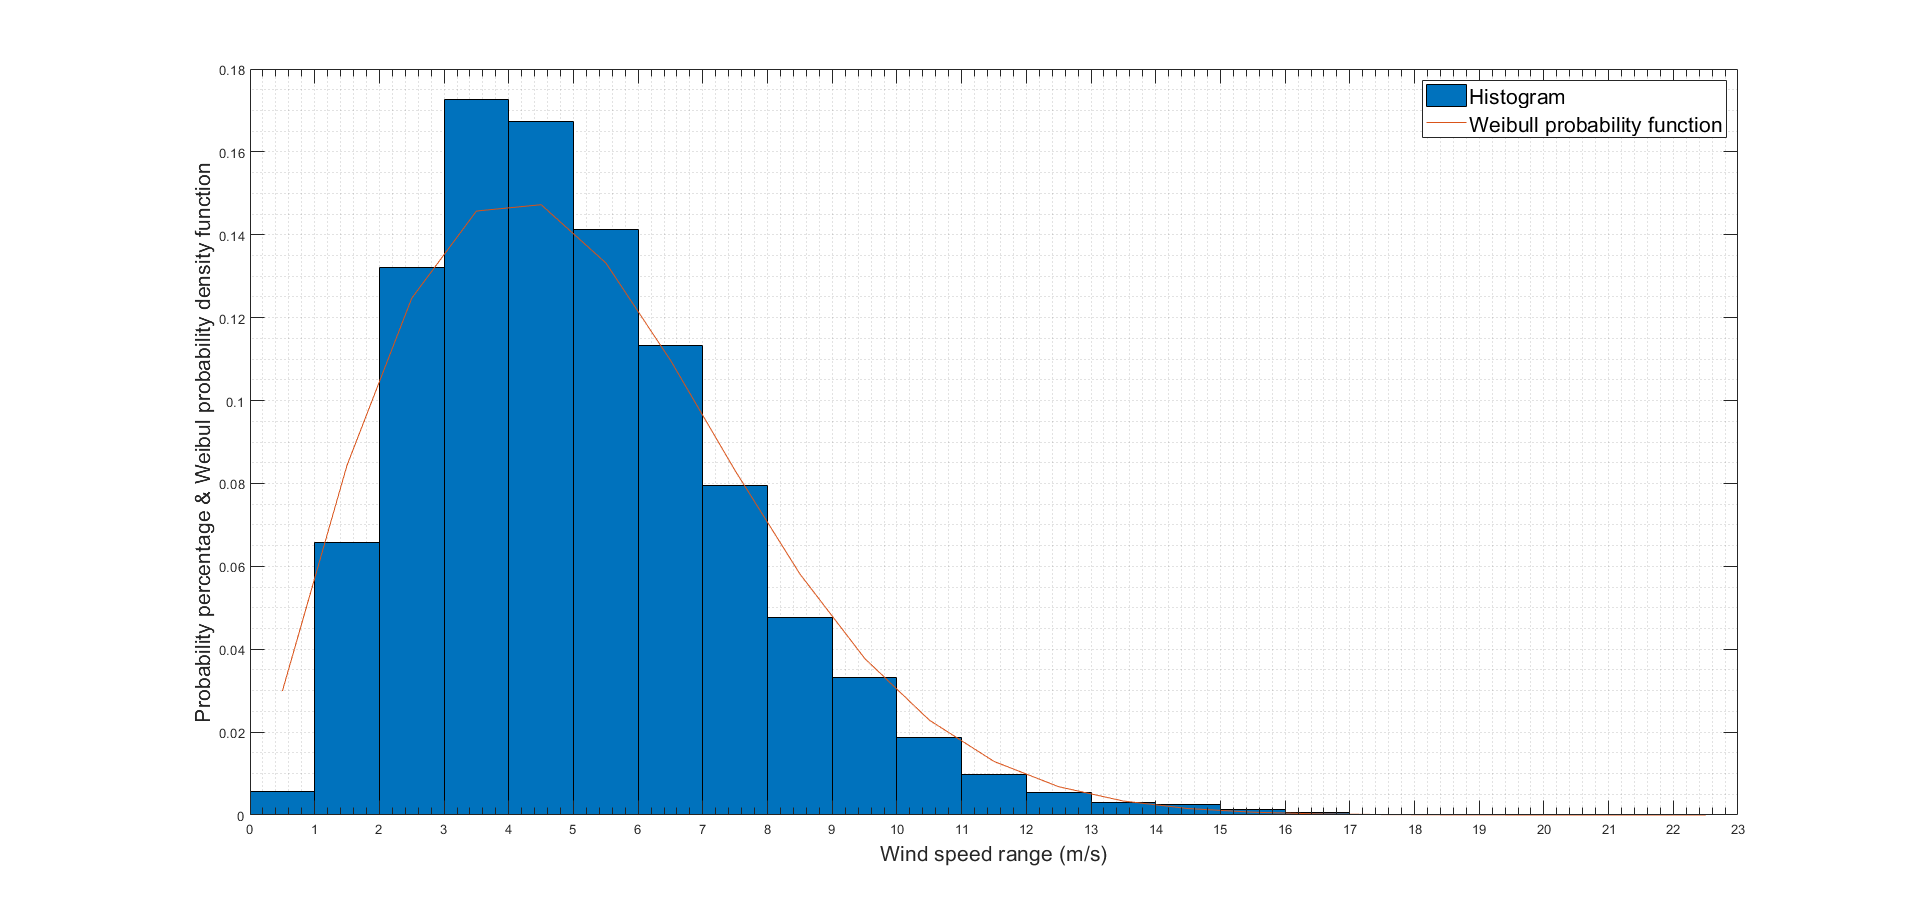
\includegraphics[width=1.1 \linewidth]{Final_report/Images/Hist.png}
    \caption{Wind climate histogram, and Weibull for Leeuwarden}
    \label{fig:hist}
\end{figure}

\newpage

\subsection{System sizing}

The initial sizing for the primary, secondary and battery was done based on the average values and the peak values of the load over the week. As seen from the initial sizing report the power ratings were oversized. After implementation of the control strategy we were able to optimize the power ratings of our sources and hence we modified our choices. The final design choices are presented in table below.


\begin{table}[H]

\begin{tabular}{|l|l|l|l|l|l|}
\hline
\textbf{Parameters}   & \textbf{Average load}  & \textbf{Peak load}     & \textbf{Primary source} & \textbf{Secondary source} & \textbf{Batteries}                                                                                                          \\ \hline
\multirow{2}{*}{Size} & \multirow{2}{*}{17 KW} & \multirow{2}{*}{47 KW} & \multirow{2}{*}{50 KW} & \multirow{2}{*}{20 KW}    & \multirow{2}{*}{\begin{tabular}[c]{@{}l@{}}12 VRF batteries(48 V, 115 Ah)\\ SOC: 20$\%$(min) to 95$\%$(max)\end{tabular}} \\
                      &                        &                        &                         &                           &                                                                                                                             \\ \hline
\end{tabular}

\end{table}

\vspace{15mm}

\section{Models used in the micro-grid}
% 3 pages
\subsection{Primary source model: Wind turbine}
The primary source is modelled in Simulink as shown in Figure \ref{fig:primary_source_model}

\begin{figure}[H]
    \centering
    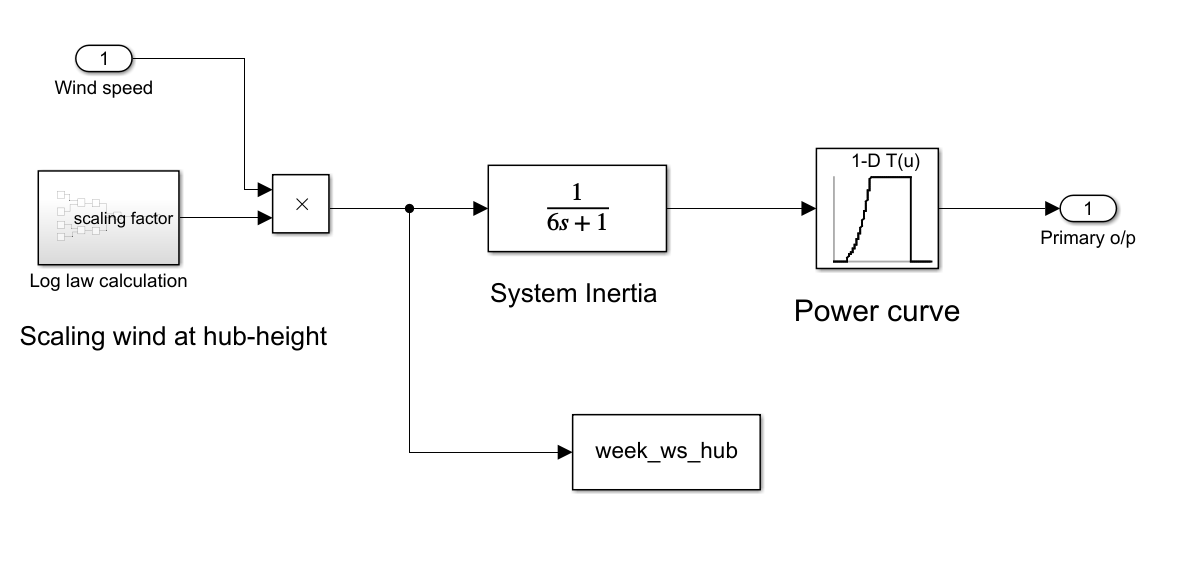
\includegraphics[width =0.6 \linewidth ]{Final_report/Images/primary_source_model.PNG}
    \caption{Primary source model}
    \label{fig:primary_source_model}
\end{figure}



\noindent The per second wind speed data of the whole week has been scaled up to the hub height of the wind turbine to calculate the power out put. Logarithmic law is used to scale the wind speed from 10m (measured height) to 35m (hub height) as shown in Equation \ref{log_law}. 

\begin{equation}\label{log_law}
    U(h)=U(ref)\frac{ln\frac{h}{z}}{ln\frac{h_{ref}}{z_{ref}}}
\end{equation}
\noindent where, U is the wind speed, h is the hub height, $h_{ref}$ is the height at which wind speed is measured, z is surface roughness at location and $z_{ref}$ is the reference surface roughness.

\begin{figure}[H]
    \centering
    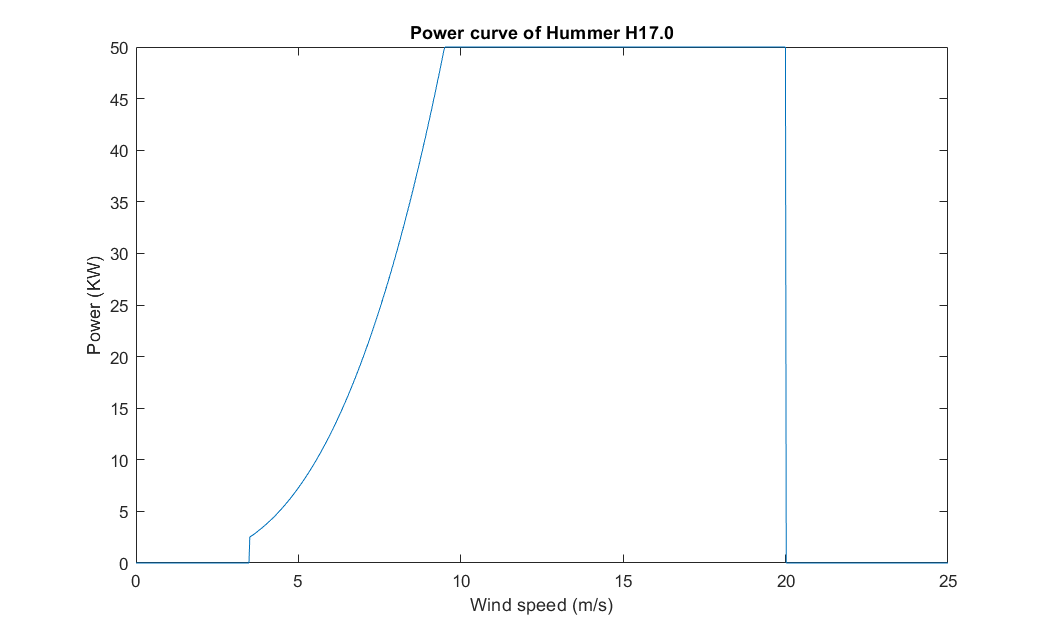
\includegraphics[width = 0.6 \linewidth]{Final_report/Images/power_curve_hummer.png}
    \caption{Power curve of Hummer H17.0}
    \label{fig:power_curve}
\end{figure}

\noindent As evident from Figure \ref{fig:primary_source_model}, the wind speed values are used to find the power output of the wind turbine using a 'look-up table' in simulink. The look-up table is the power curve of the turbine which gives the power output at the particular wind speed. To model the system inertia of the wind turbine, a transfer function is used with a value of 6 seconds scaled using the proportionality relation in \citep{Tang2008}. The output from the look-up table is then used further in the central controller to calculate the mismatch.
%insert citation of inertia value



\subsection{Secondary source model: Biomass plant}
%S
The secondary source is modelled in Simulink as given below:
\begin{figure}[H]
    \centering
    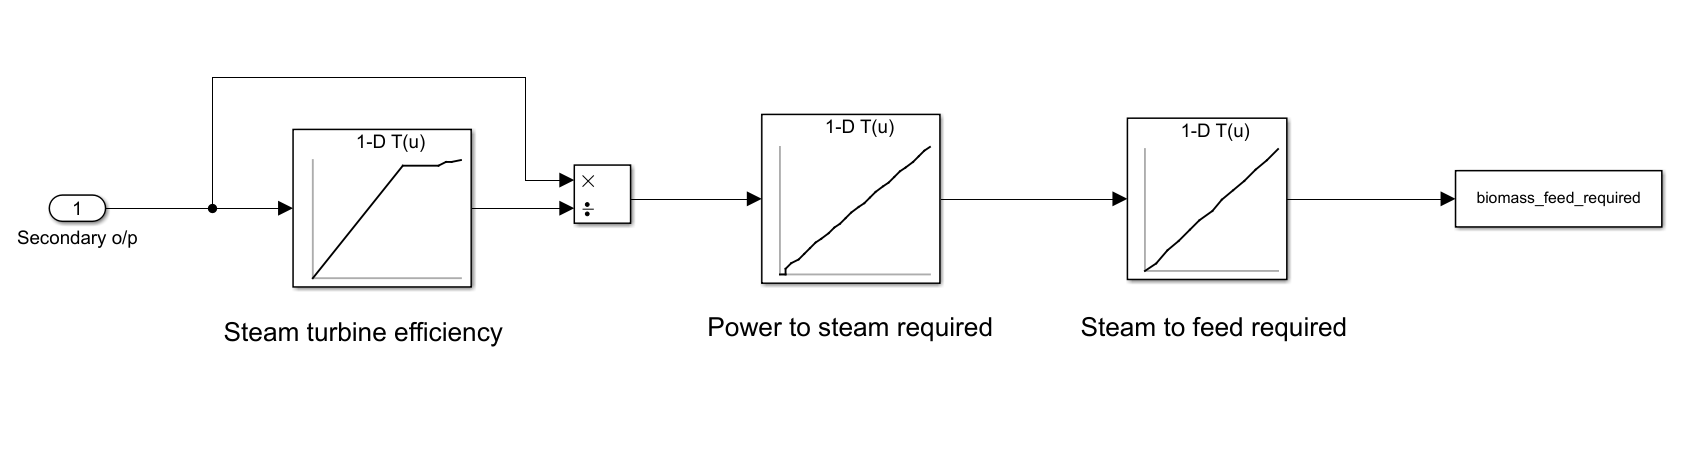
\includegraphics[width = 0.9 \linewidth]{Final_report/Images/feed_calculations.PNG}
    \caption{Secondary source model}
    \label{fig:secondary model}
\end{figure}

\noindent The model calculates the amount of torrefied biomass (feedstock)  required to produce the power to cater to secondary source load. The variable efficiency for biomass power plant considered is the electrical efficiency of steam turbine, which can be defined a function of secondary source load \citep{karakurt}, as shown in Figure \ref{fig:SteamEff}. 

\begin{figure}[H]
    \centering
    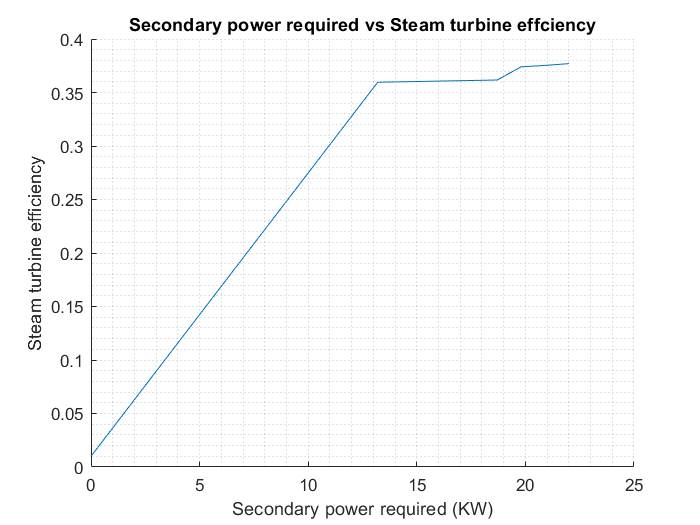
\includegraphics[width = 0.5 \linewidth]{Final_report/Images/steam_tur_eff.png}
    \caption{Steam turbine efficiency as function of secondary load}
    \label{fig:SteamEff}
\end{figure}



This efficiency is used to convert the load to biomass plant output power as shown in Equation \ref{Turbineeff}. 

\begin{equation}\label{Turbineeff}
   Biomass\ \ O/P = \frac{Secondary\ \ O/P}{Turb_{Eff}}
\end{equation}
\newline
where 
\newline Biomass\ \ O/P is the biomass plant power output
\newline Secondary\ \ O/P is the secondary source load
\newline {$Turb_{Eff}$} is the steam turbine efficiency
\newline

\noindent Further, the steam flow rate followed by feed flow rate required is estimated using 'Power to steam'  and 'Steam to feed' look up tables respectively as shown in Figure \ref{fig:P_to_S} and Figure \ref{fig:S_to_B}.


\begin{figure}[H]
\begin{subfigure}{.5\textwidth}
  \centering
  % include first image
  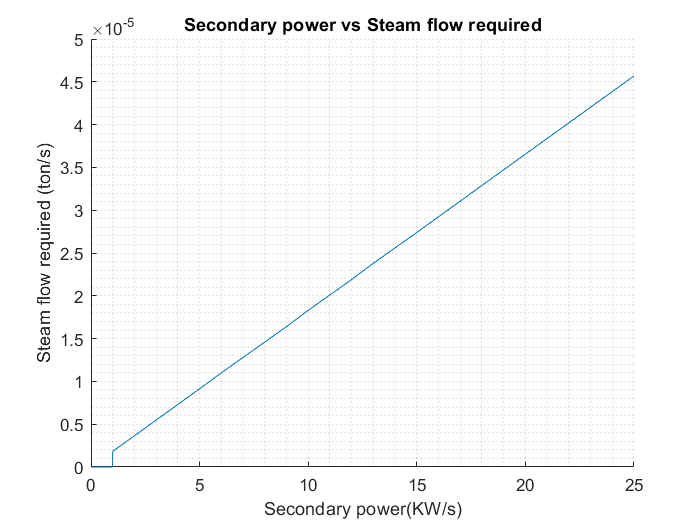
\includegraphics[width=.8\linewidth]{Final_report/Images/power_to_steam_req.png}
  \caption{Power to steam flow-rate required}
  \label{fig:P_to_S}
\end{subfigure}
\begin{subfigure}{.5\textwidth}
  \centering
  % include second image
  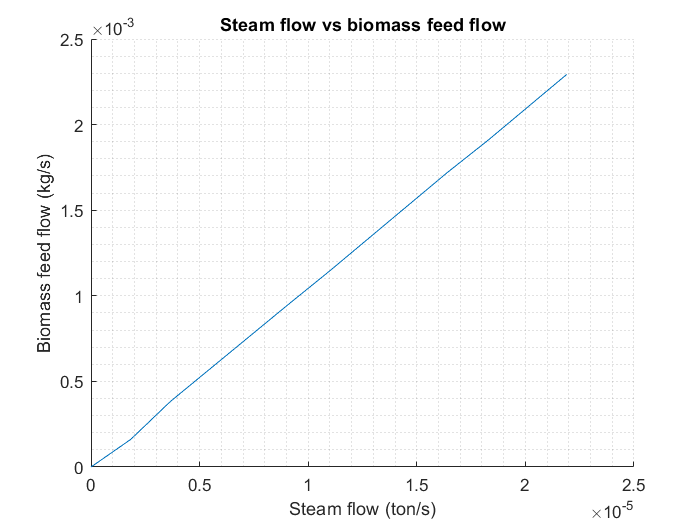
\includegraphics[width=.8\linewidth]{Final_report/Images/steam_to_biomass.png}  
  \caption{Steam flow rate to torrified biomass flow rate required}
  \label{fig:S_to_B}
\end{subfigure}
\caption{Calculation of biomass feed}
\label{fig:calculation_feed}
\end{figure}

\noindent The look-up table data calculations were done on basis of steam turbine and boiler equations stated in the steam system modeler provided by \citep{advanced}.The biomass flow rate thus calculated is taken into consideration while estimating the LCOE in Section \ref{sec:eco}. 


\subsection{Battery}

The variable efficiencies considered for redox flow batteries are the battery system efficiency and battery energy efficiency. While battery energy efficiency refers to the discharge capacity efficiency of the battery, battery system efficiency is the overall system efficiency which includes discharge efficiency, pumping losses and frictional losses. Based on the literature \citep{bryans_amstutz_girault_berlouis_2018} \citep{7110861},the efficiencies are plotted as function of state of charge (SOC) as follows:

\begin{figure}[H]
\begin{subfigure}{.5\textwidth}
  \centering
  % include first image
  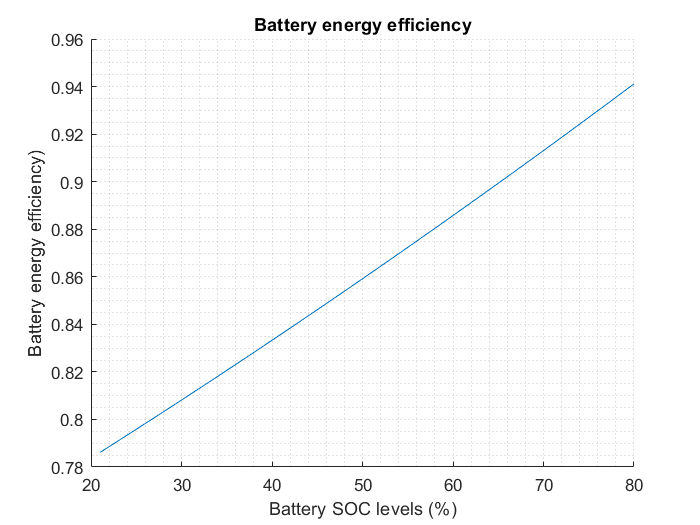
\includegraphics[width=.8\linewidth]{Final_report/Images/battery_energy_efficiency.png}
  \caption{Battery energy efficiency as a function of SOC}
  \label{fig:BatEnergy}
\end{subfigure}
\begin{subfigure}{.5\textwidth}
  \centering
  % include second image
  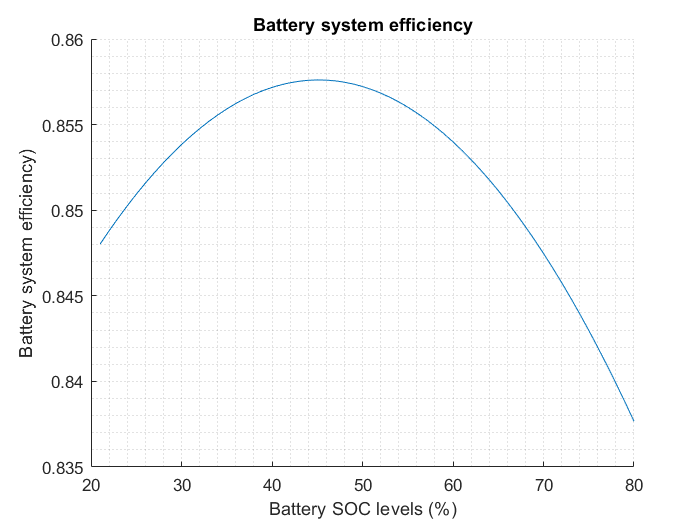
\includegraphics[width=.8\linewidth]{Final_report/Images/battery_system_efficiency.png}  
  \caption{Battery system efficiency as function of SOC}
  \label{fig:BatSys}
\end{subfigure}
\caption{Battery Variable Efficiencies}
\label{fig:calculation_feed}
\end{figure}
\newline
The battery SOC calculation model is given as:

\begin{figure}[H]
    \centering
    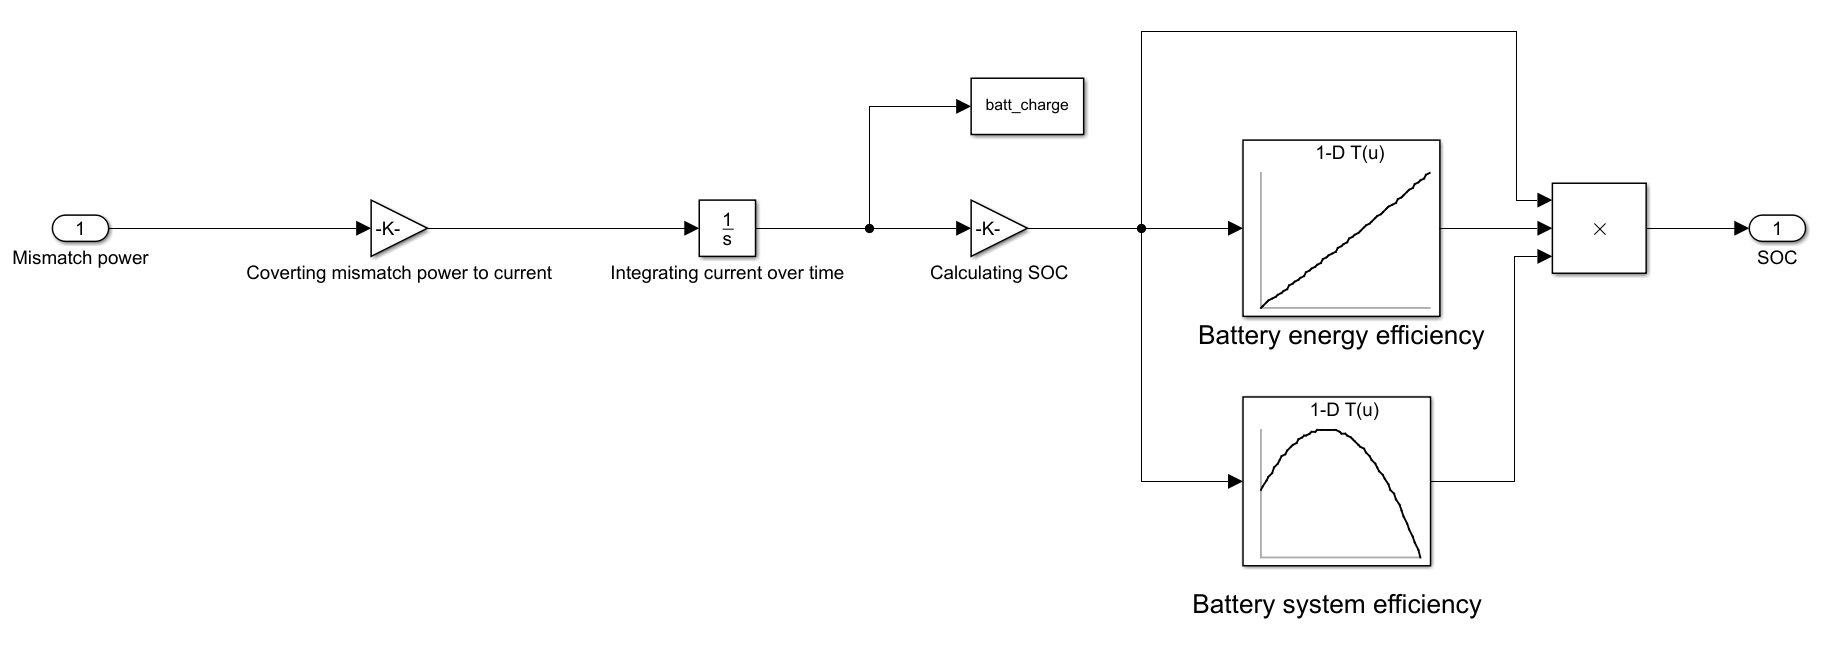
\includegraphics[width = 0.9 \linewidth]{Final_report/Images/batt_soc_calc.PNG}
    \caption{Battery SOC calculation}
    \label{fig:BatSOC}
\end{figure}

From Figure \ref{fig:BatSOC}, it can be observed that the mismatch power is converted to current and integrated over time to get the total current capacity (Ampere second). SOC is further calculated by Equation \ref{SOCcalc}.

\begin{equation}\label{SOCcalc}
   SOC_{final} = \frac{Total\ \ Current \ \ Capacity}{n.Batcap.3600}.E_{eff}. Sys_{eff}
\end{equation}
\newline 
where Batcap is the battery capacity(Ah)
\newline where n is the number of batteries
\newline where Total\ Current\ Capacity is the total mismatch power in terms of battery capacity(As)
\newline where $E_{eff}$ is the energy efficiency of battery which is obtained from lookup table of Fig. \ref{fig:BatEnergy}
\newline where  $Sys_{eff}$ is battery system efficiency from lookup table of Fig. \ref{fig:BatSys}. \newline

\noindent Hence, this SOC value is updated in the central controller block. The battery control is further elaborated in section \ref{sec:control}. 
 

\newpage


\section{Control}  \label{sec:control}

This section describes the overall control philosophy of the microgrid and the justification for the choice of the control.\\

\noindent The control philosophy adapted in the model is an hybrid in nature. The microgrid central controller is responsible for interacting with the work space and local primary, secondary and battery control. This architecture is built to emulate the real life I/O block (data link layer) in the central control wherein the central controller receives the Input from the field signal and then sends it to the target device to be controlled. The primary, secondary, and battery have their individual controllers, which decide the state of their individual production, depending on the input from the microgrid central controller.The central controller is also responsible for the scheduled maintenance of the wind turbine. In the case of a sudden failure of the secondary  \\

\noindent After the justification of the control architecture,in the following section  the control strategy shall be discussed in detail. \\

\subsection{Primary control:}
The controller can be visualised from \ref{fig:primary_source_model}
The data link layer in the central controller
receives the per second wind speed data at the location, and sends it to the  controller of the primary source. In the primary control, the wind speed is converted to the wind speed at the hub height of the turbine using the log law equation. This is followed by a delay in order to simulate the inertia of the turbine.The chosen value of time constant $ \tau $ for the delay is 6 seconds.

\noindent Subsequently the the maintenance signal from the central control is checked. If there is no signal of maintenance then the power produced by the turbine is calculated on the basis of the wind speed at the hub. If the wind speed is below the cut in, above the cut out speed the primary controller switches off the turbine. The power produced by the turbine is further transferred to the central controller. 

\subsection{Secondary control:}
\begin{figure}[H]
    \centering
    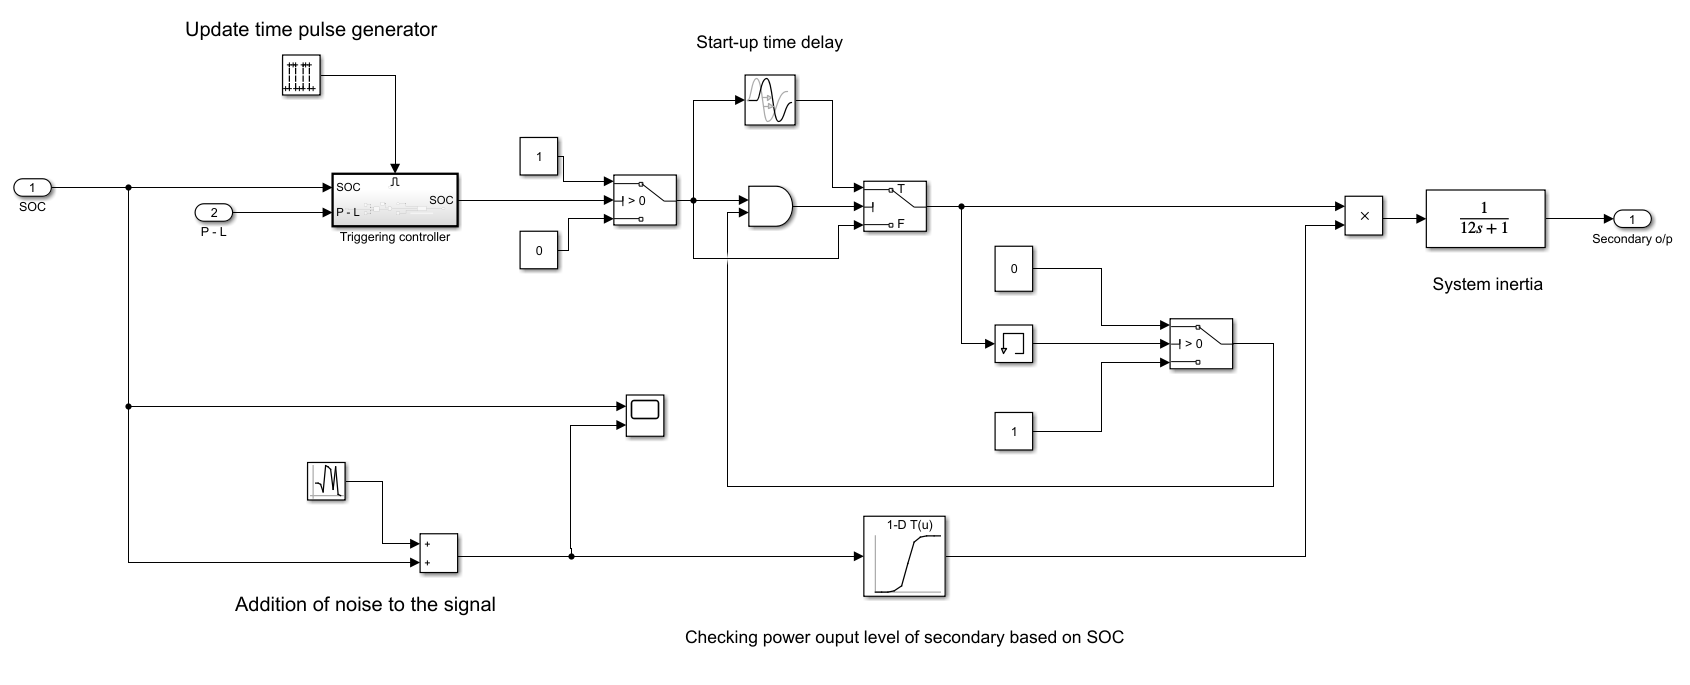
\includegraphics[width = 1 \linewidth]{Final_report/Images/secondary_source_controller.PNG}
    \caption{Secondary source controller}
    \label{fig:seconday_source_controller}
\end{figure}

The secondary control can be visualized from \ref{fig:seconday_source_controller}.
\noindent The secondary source is a controllable source and hence it is dispatched only if the need arises, i.e. is not continuous in nature. The input parameters for the secondary control are the difference between the instantaneous primary generation and load. These are provided by the central controller. Inside the secondary control there is an update time block which updates the state of the secondary generation. The update time is nothing but a pulse generator with a frequency of 0.27 mHz (once every hour), and the pulse width is 1s.

\noindent At the instance of the pulse, the controller checks whether the difference between the instantaneous primary generation and load is negative or positive. If the difference is positive then the controller takes no action. But, if it is negative, then it checks the previous state of the secondary generation which is stored in the memory block. If the value is zero then it delays the starting signal of secondary by 40 minutes. This is done in order to emulate the cold/warm starting time of a steam turbine. If the value of the memory is greater than zero then the start signal is instantly generated. 
%secondary triggering condition with SoC 0.7. reason?
Subsequently the level of generation of the secondary is decided based on the SOC of the battery, the levels are specified in the \ref{table:Power_level}.This restricts the switching on of the secondary source when there is just a instantaneous negative mismatch between the primary generation and the load. Hence saving up on fuel costs by considering the wholesome state of the system. The value of secondary generation is then passed to the central controller.
\begin{table}[h]
\centering
\caption{Secondary Power level corresponding to SOC}
\begin{tabular}{|l|l|} 
\hline
SOC                  & Power(kW)             \\ 
\hline
0.3-0.4              & 20                    \\ 
\hline
0.4-0.5              & 15                    \\ 
\hline
0.5-0.6              & 9                     \\ 
\hline
0.6-0.7              & 4                     \\ 
\hline
0.7-0.95             & 0                     \\ 
\hline
\multicolumn{1}{l}{} & \multicolumn{1}{l}{} 
\end{tabular}
\end{table}\label{table:Power_level}
\subsection{Battery:}
The battery controller receives,the instantaneous difference between the primary, secondary generation and the load from the central controller. The mismatch between primary plus secondary minus load (P+S-L) is chosen in order to prevent the charging of the battery using the secondary source. If there is an instantaneous mismatch and the SOC of the battery is above 0.2 then the battery discharges and provides the instantaneous power to maintain the balance.
In the case of positive mismatch the battery is charged until and unless the SOC of the battery is below 0.95.
The SOC of the battery plays an important role in the secondary control and hence the SOC is passed to the central controller, which further passes it to the secondary controller.

\subsection{Microgrid central controller:}
Depending on the user input it decides the maintenance of the wind turbine, sudden breakdown of the secondary generation or a variation in the load. The relevant signals are then passed to the respective local controllers.
The central controller generates the instantaneous difference between the primary, secondary generation and load. It further sends it to the local primary, secondary and battery controller for their local control. The central controller receives the SOC of the battery and further passes it to the secondary controller.The control can be visualized from the \ref{fig:central_control}.
\begin{figure}[H]
    \centering
    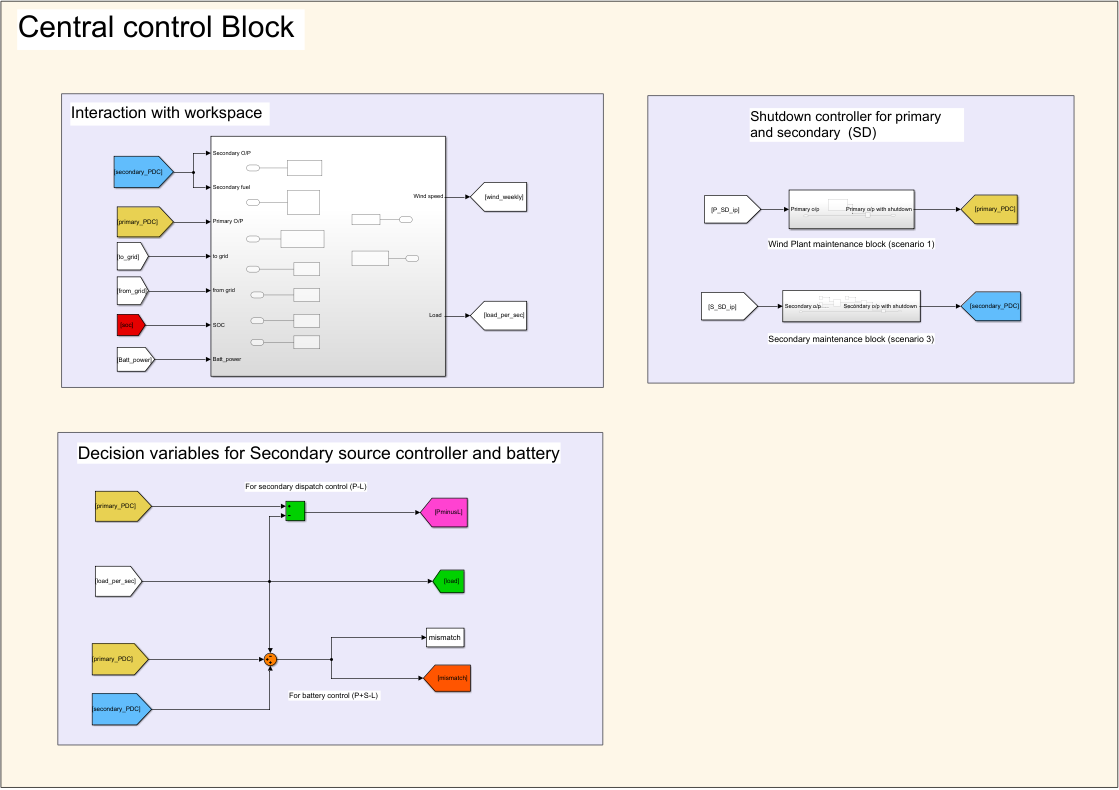
\includegraphics[width = 0.8 \linewidth]{Final_report/Images/central_controller.PNG}
    \caption{Central controller}
    \label{fig:central_control}
\end{figure}

\noindent The flow chart mentioned in Figure 1 of Progress report remains aligned with the control philosophy, the addition to this was the introduction of the scenario controller, to simulate the scenarios provided. The \ref{fig:scenario_control} depicts the flow of the logic of the scenario controller. The output of this then goes to the fig 1. progress report and then the flow continues.
\begin{figure}[H]
    \centering
    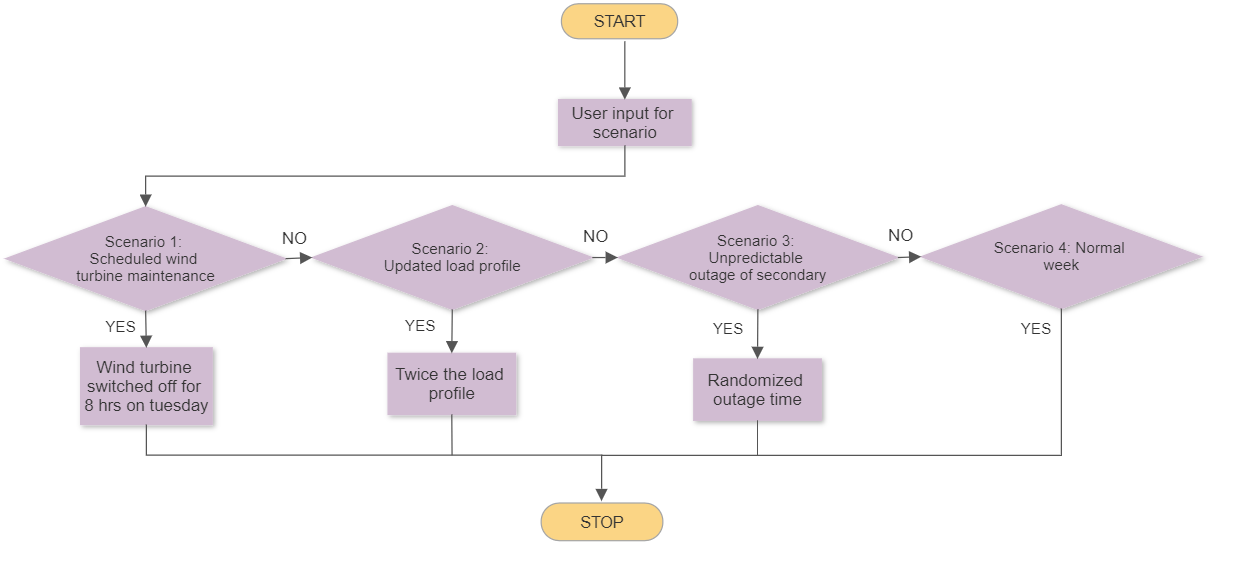
\includegraphics[width = 0.8 \linewidth]{Final_report/Images/Scenario_Controller.PNG}
    \caption{Flow chart of scenario controller}
    \label{fig:scenario_control}
\end{figure}

\newpage

\section{Simulation results of normal week and scenarios} \label{sec:simulation_plots}
In this section, the simulation results are plotted for all the scenarios and their impacts are discussed in section \ref{scenario_discussion}.

\begin{figure}[H]
    \centering
    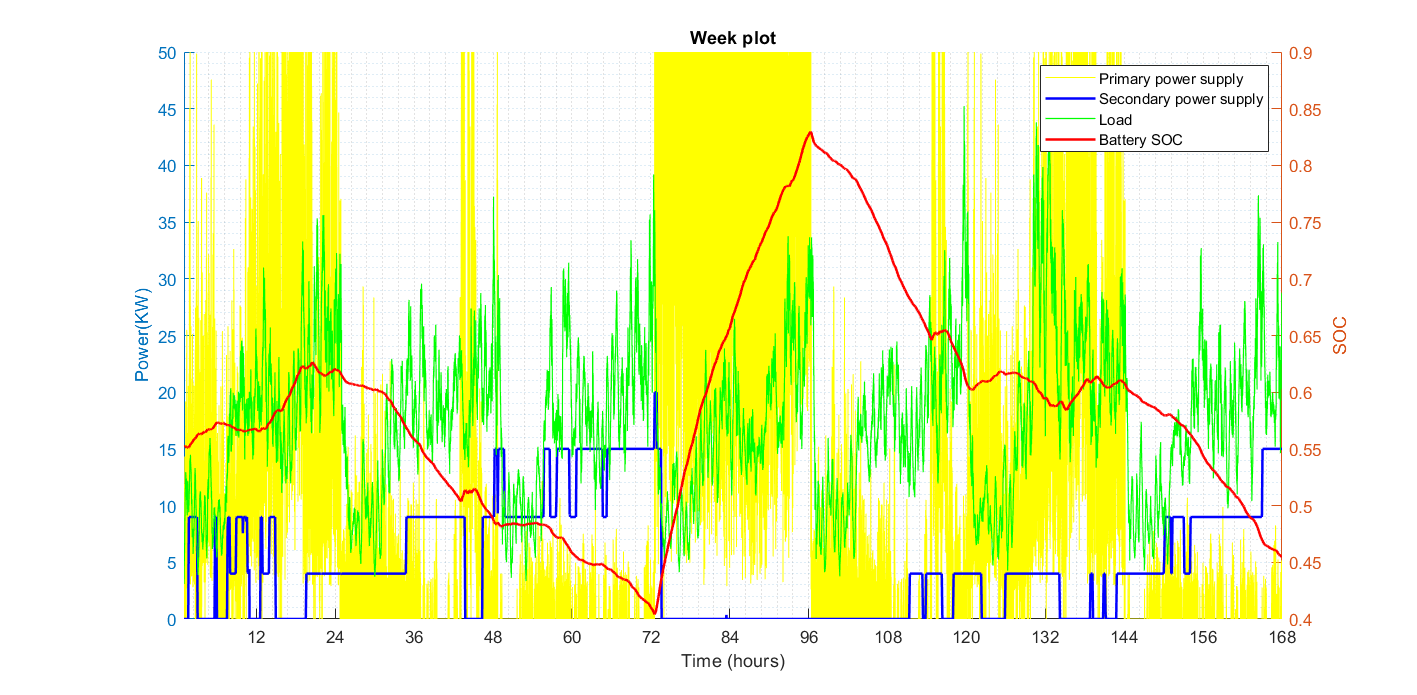
\includegraphics[width=1 \linewidth]{Final_report/Images/Week_plot_normal.png}
    \caption{Week plot of normal scenario}
    \label{fig:week_plot_normal}
\end{figure}

\begin{figure}[H]
    \centering
    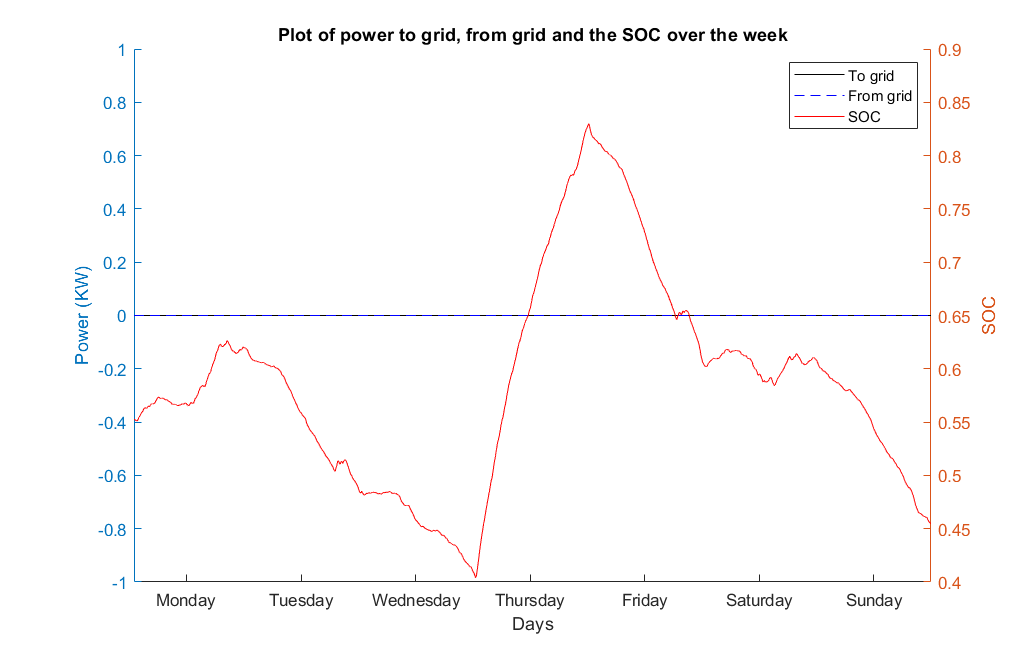
\includegraphics[width=0.7 \linewidth]{Final_report/Images/to_from_SOC_normal.png}
    \caption{Grid exchange for normal week}
    \label{fig:grid_ex_normal}
\end{figure}

\begin{figure}[H]
    \centering
    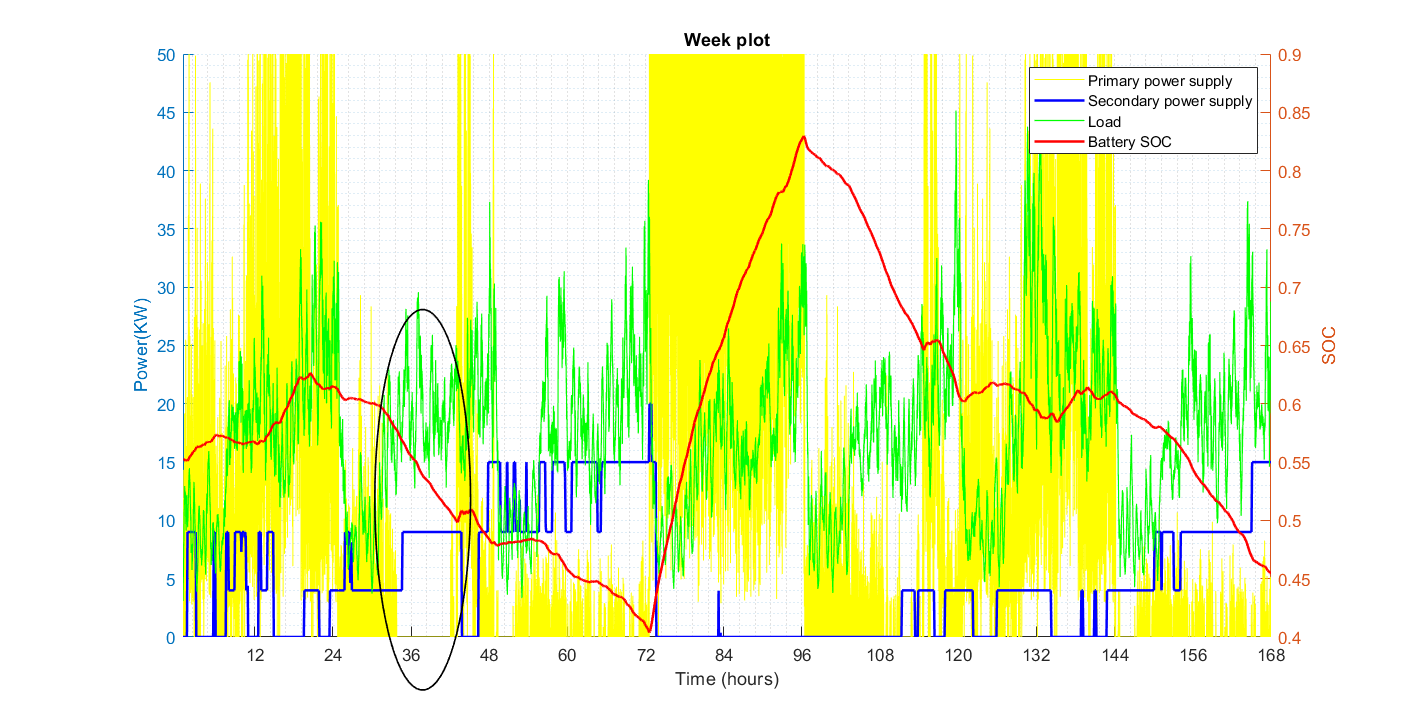
\includegraphics[width=1 \linewidth]{Final_report/Images/Week_plot_s1.png}
    \caption{Week plot of scenario 1 (Scheduled maintenance of wind turbine on Tuesday for 8 hours)}
    \label{fig:week_plot_s1}
\end{figure}

\begin{figure}[H]
    \centering
    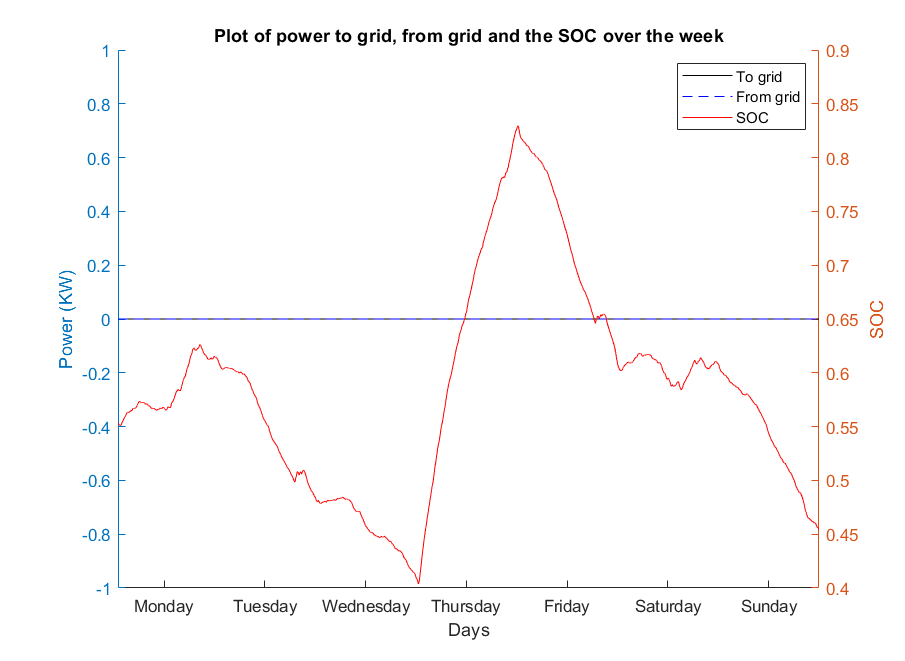
\includegraphics[width=0.7 \linewidth]{Final_report/Images/to_from_SOC_s1.png}
    \caption{Grid exchange for scenario 1}
    \label{fig:grid_s1}
\end{figure}

\begin{figure}[H]
    \centering
    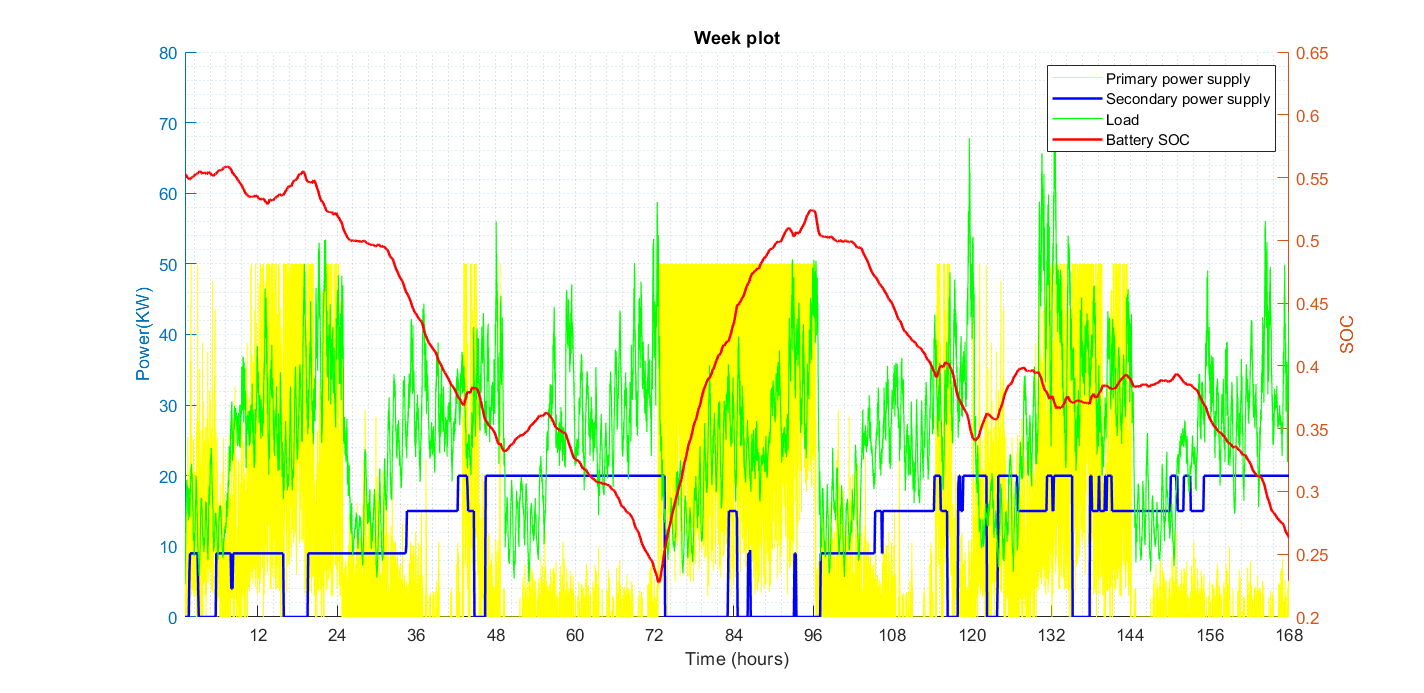
\includegraphics[width=1 \linewidth]{Final_report/Images/Week_plot_s2.png}
    \caption{Week plot of scenario 2 (Load variation)}
    \label{fig:week_plot_s2}
\end{figure}

\begin{figure}[H]
    \centering
    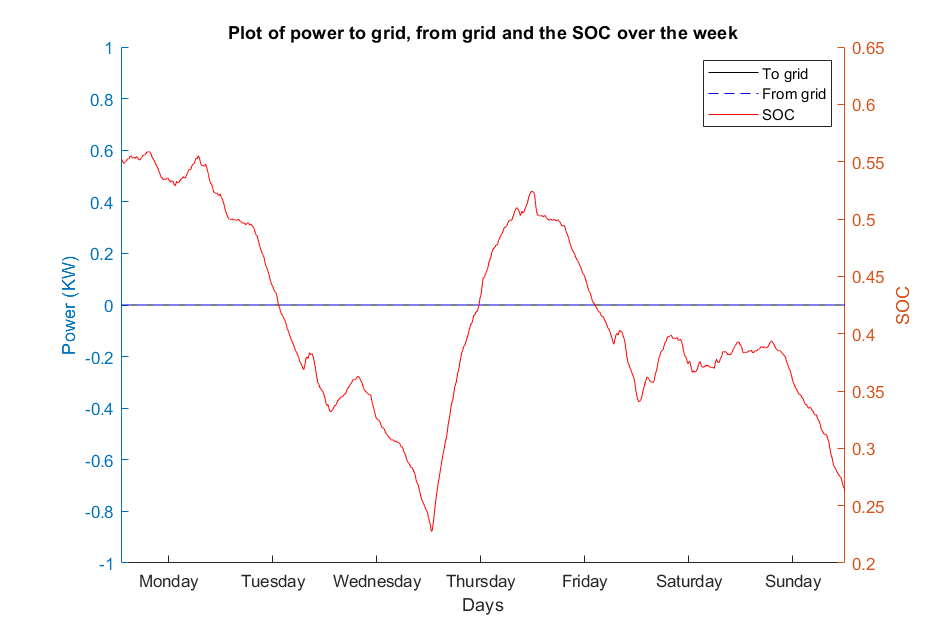
\includegraphics[width=0.7 \linewidth]{Final_report/Images/to_from_SOC_s2.png}
    \caption{Grid exchange for scenario 2}
    \label{fig:grid_s2}
\end{figure}

\begin{figure}[H]
    \centering
    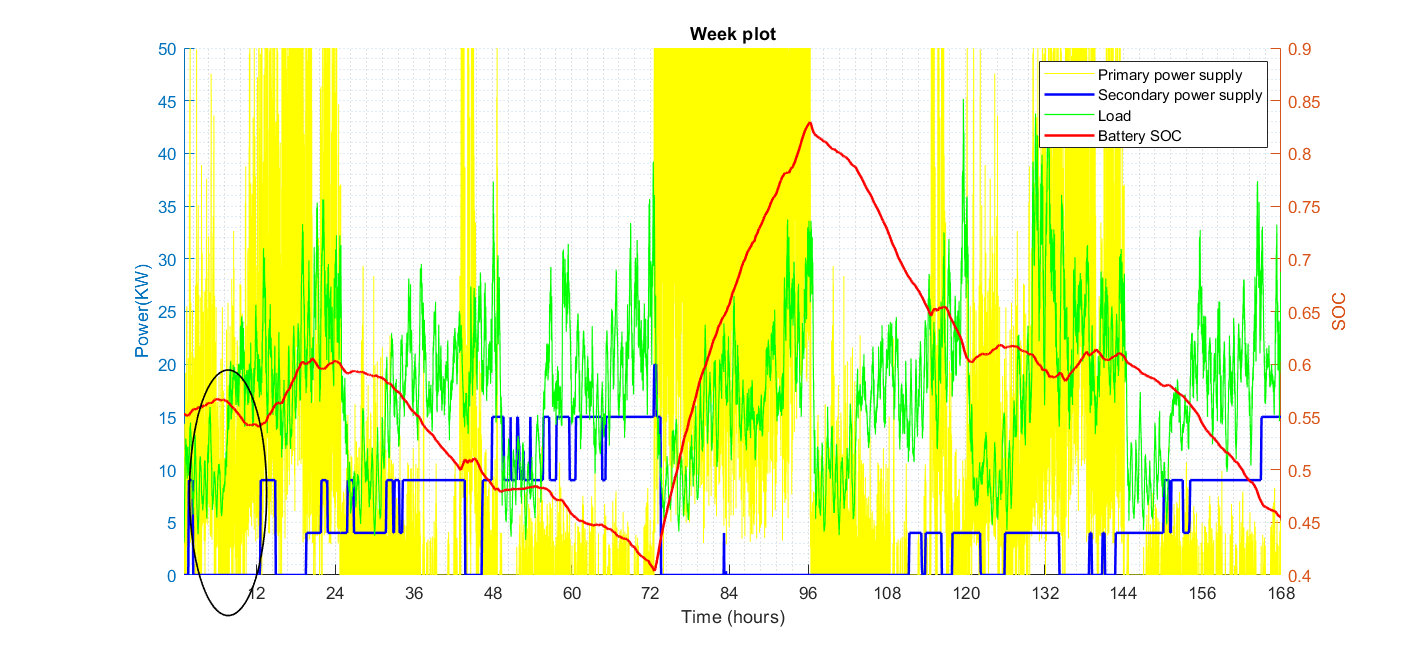
\includegraphics[width=1 \linewidth]{Final_report/Images/Week_plot_s3.png}
    \caption{Week plot of scenario 3 (Secondary plant shutdown due to unpredictable cause)}
    \label{fig:week_plot_s3}
\end{figure}

\begin{figure}[H]
    \centering
    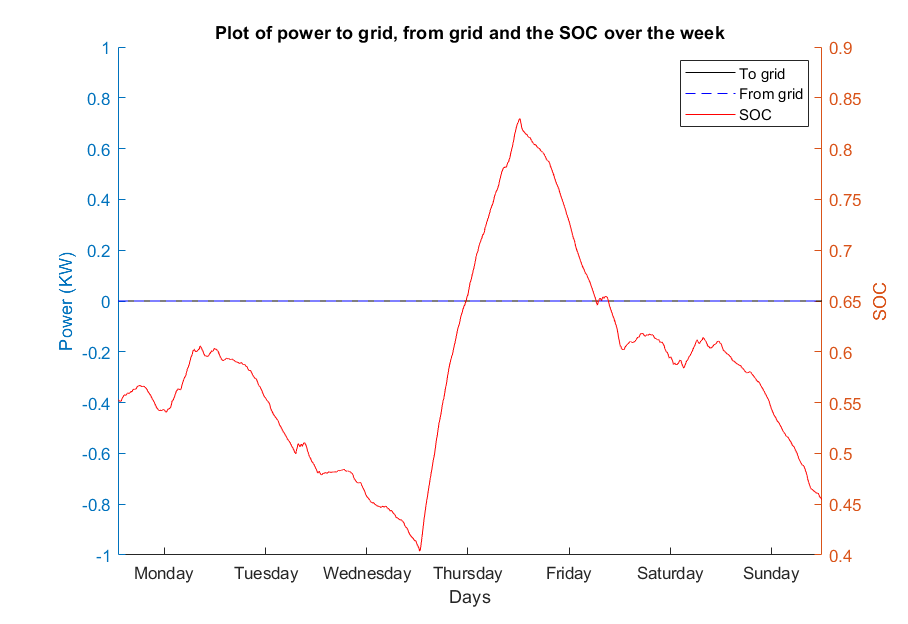
\includegraphics[width=0.7 \linewidth]{Final_report/Images/to_from_SOC_s3.png}
    \caption{Grid exchange for scenario 3}
    \label{fig:grid_s3}
\end{figure}

\section{Three scenarios and discussion on their impacts } \label{scenario_discussion}

All the 3 scenarios have been explained in this section. Section \ref{sec:simulation_plots} gives the simulation results of the scenarios. As evident from the plots, it can be inferred that the designed micro-grid is robust and it does not have any exchange with the grid in all the scenarios.

\subsection{Scenario 1: Scheduled maintenance of wind turbine}
This scenario is modelled to test if our micro-grid is sustainable without any exchange with the grid in situations when the wind turbine is under maintenance. As evident from Figure \ref{fig:week_plot_s1}, the maintenance is scheduled on Tuesday for 8 hours. The number of hours chosen align with a standard service shift for wind turbine maintenance/repairs. The turbine is shutdown by sending a signal to the shutdown controller which is a part of the central controller for the micro-grid. As seen from the graph, the secondary source automatically ramps up to cater the load in absence of the primary source. Immediately when the primary source is back online, the secondary controller is shutdown based on the mismatch and the battery state of charge. The working of secondary controller is explained in detail in section \ref{sec:control}. This situation may lead to an increase in the secondary feed requirement of the week than compared to a normal week.    


\subsection{Scenario 2: Load variation}
This scenario is modelled to test if our micro-grid is sustainable without any exchange with the grid in situations when the load variation is unusually higher than expected over the week. In this scenario, we have increased the load by 1.5 times the given values. As seen from Figure \ref{fig:week_plot_s2}, the maximum state of charge of the battery is around 55\% as opposed to in normal week operation where it is around 85\%. Also, the secondary source feed requirement increases substantially during such scenarios. In normal week operation the feed requirement was around 2.6 tons, whereas, it is 4 tons for this scenario. This would lead to an increase in the costs for operation of the biomass plant and hence increase the cost of energy.

\subsection{Scenario 3: Secondary plant unavailable due to unpredictable cause}
This scenario is modelled to test if our micro-grid is sustainable without any exchange with the grid in situations when the secondary power source (biomass plant) shuts down at unpredictable time and also for unpredictable period. This scenario is modelled by generating random values for shutdown time and the shutdown period. The range given for generating the random value for shutdown time is from 1 second to 604800 seconds (i.e. anytime in the week). The range given for shutdown period is from 6 hours to 12 hours. As seen from Figure \ref{fig:week_plot_s3}, The biomass plant shuts down after 1 hour from start of the week and remains shutdown for 10 hours. The SOC of the battery might be affected due to this scenario as when the biomass plant is offline along with lower wind speeds, the batteries will have to cater to the load demand for that period.




\vspace{15mm}


\section{3 phase output and discussion}
%why is battery voltage and current out of phase
%grid current zero
In this section the 3-Phase outputs for 4 cycles of voltage and current are visualized and discussed. To simulate the 3 phase grid, the load was first converted into P+jQ format by providing 0 as an input for its reactive component. The DC power output of the batteries is converted into 3 phase output with the help of an inverter. The primary and secondary generations are also converted into 3 phase outputs and then all these components are connected to the 3 phase grid. Figure \ref{fig:3ph_grid_batt} depicts the 3 phase voltages and currents of the grid side. There is presence of voltage since the the microgrid references for voltage and frequency from the grid. The color code standards for the 3 phases i.e. RYB is followed, the phase sequence is (0,120,-120). Since the constraint of grid exchange to be zero is a required, as observed, there is no flow of current to or from the grid.This zero current proves that the model confirms with the requirement.
\begin{figure}[H]
    \centering
    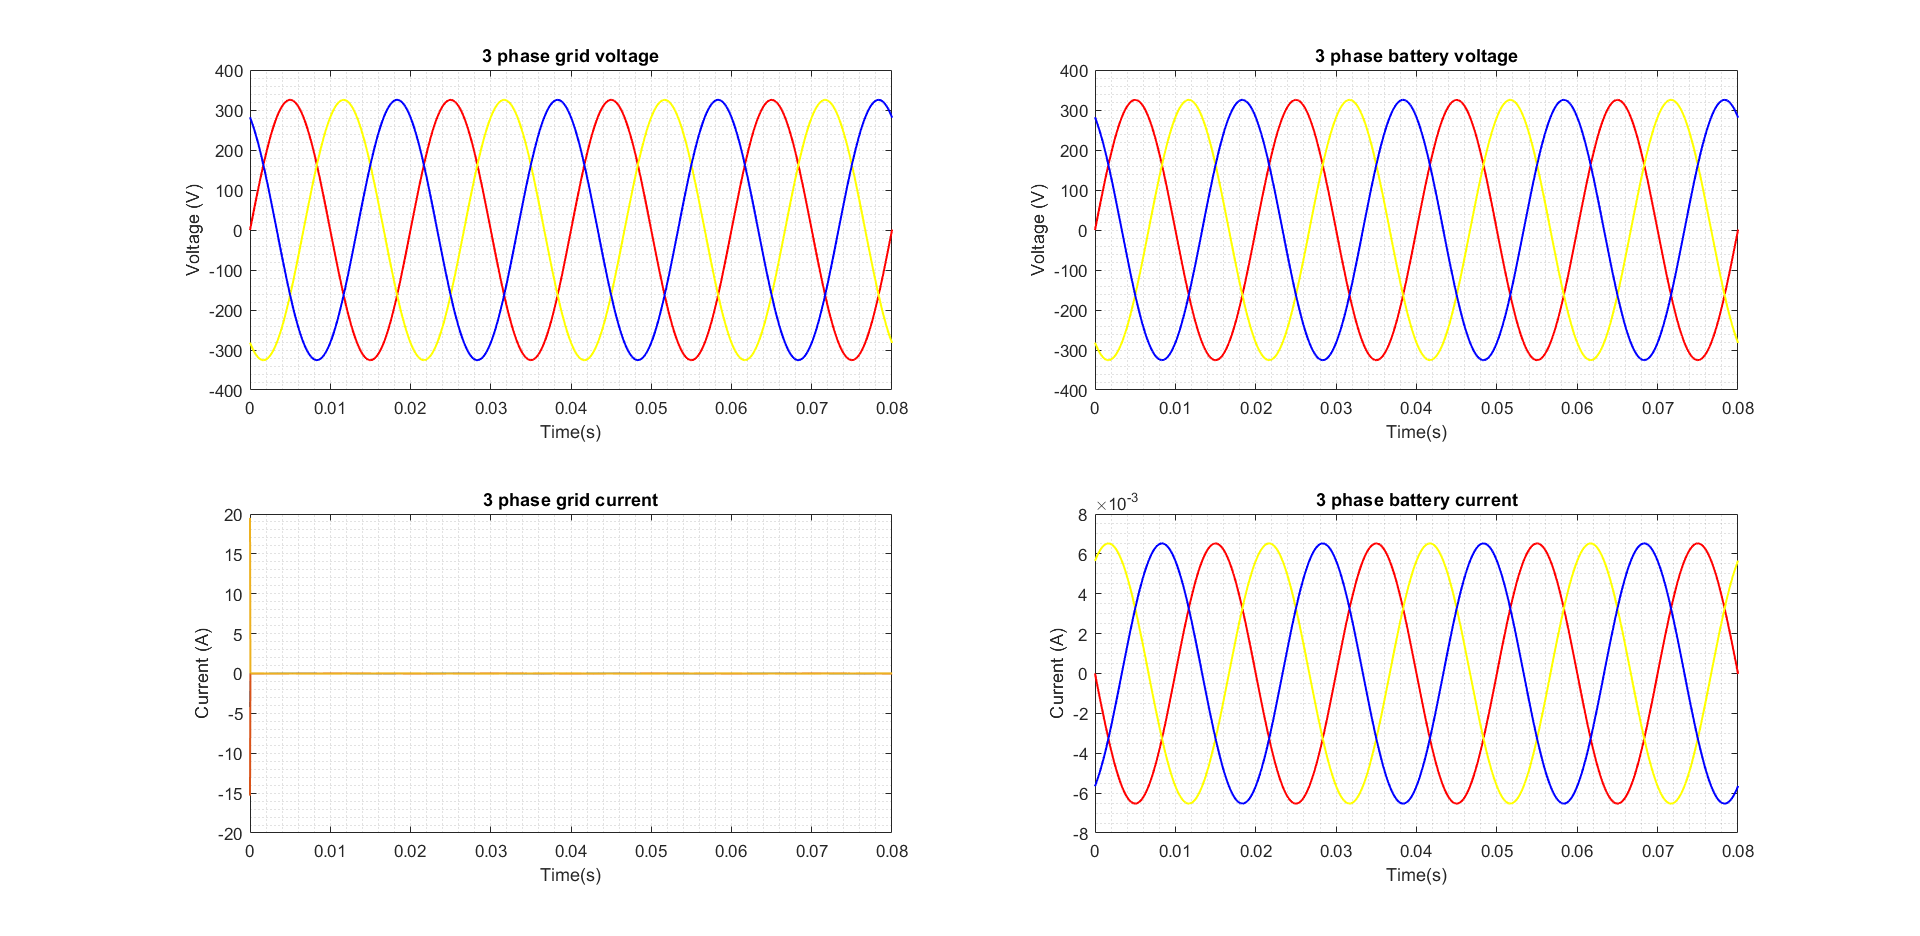
\includegraphics[width=1.1 \linewidth]{Final_report/Images/3ph_grid_batt.png}
    \caption{3 Phase voltages and currents(grid and battery)}
    \label{fig:3ph_grid_batt}
\end{figure}

\noindent Since the simulation has been carried out only for 4 seconds, the only source that is dispatched is the battery. It is due to the fact that the wind speeds are below cut in speed and the secondary source is not triggered as the battery SoC is above 0.7.The zero current in the \ref{fig:3ph_pri_sec} can be visulaised to reaffirm the fact stated above. 
The battery voltage and current are in phase since there are only active power  loads in the system. The current amplotude of the battery is 6 mA. The magnitude is lower since the voltage is 320 V which is the Phase to ground voltage.
\begin{figure}[H]
    \centering
    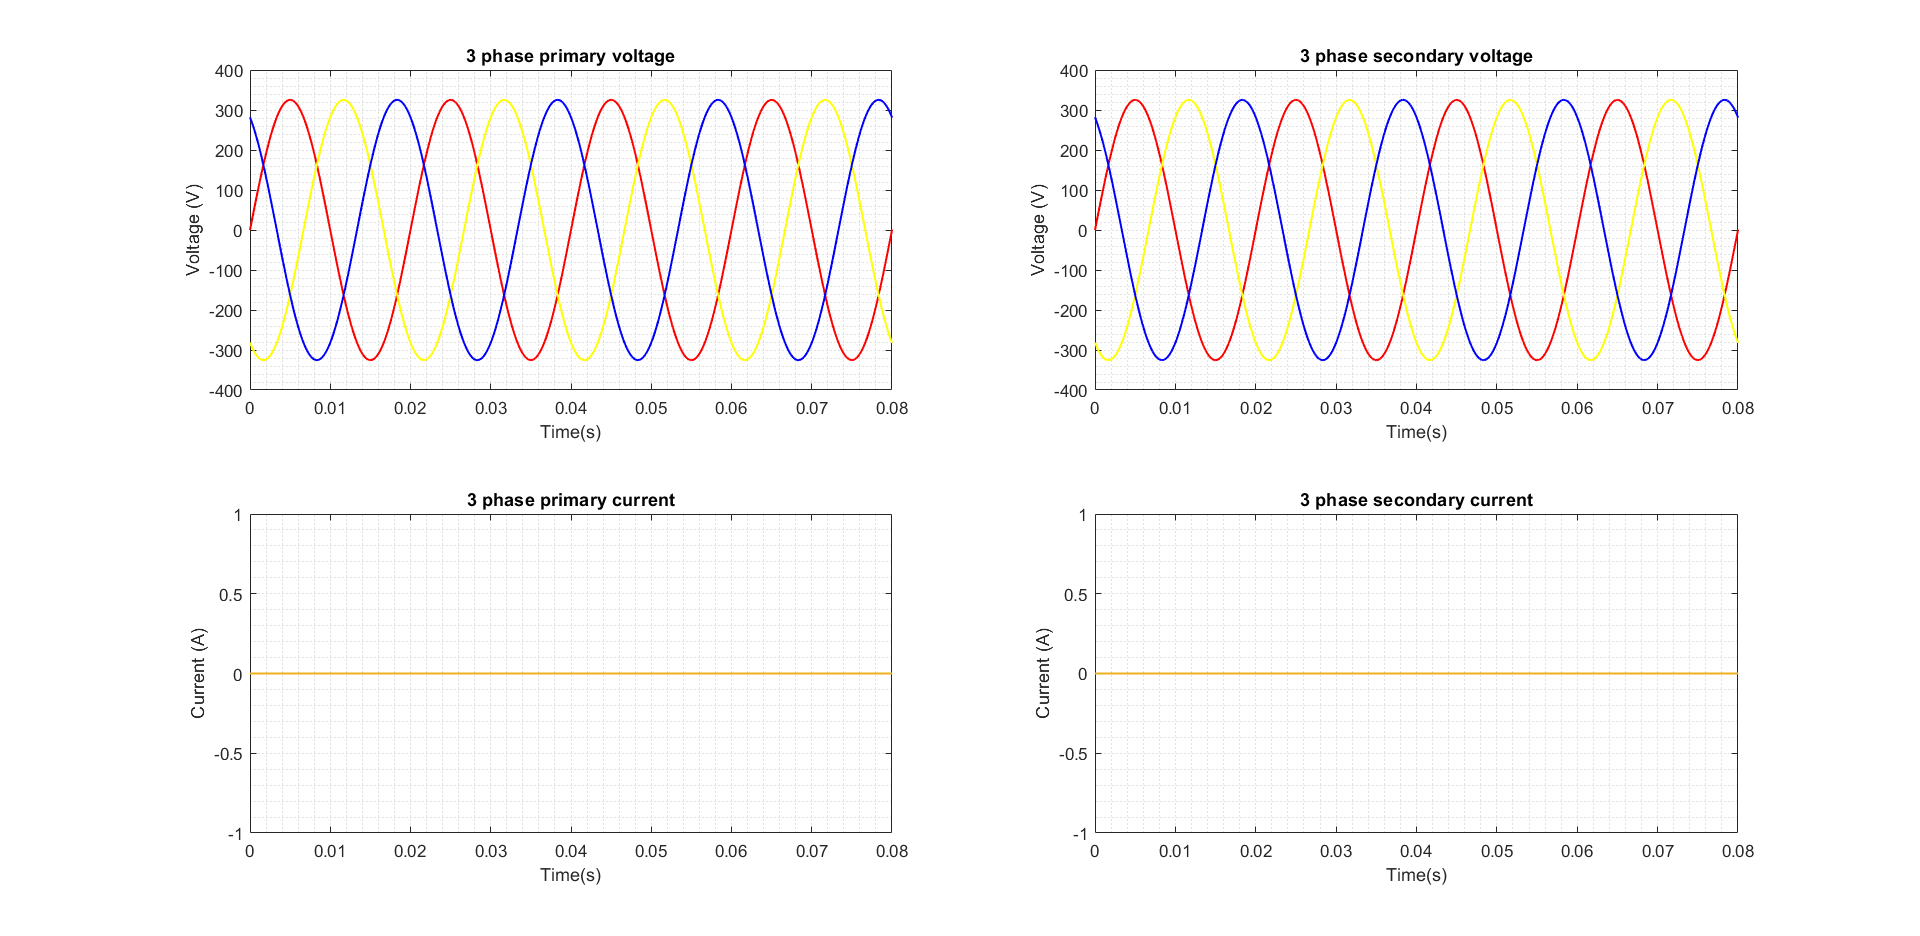
\includegraphics[width=1.1 \linewidth]{Final_report/Images/3ph_primary_secondary.png}
    \caption{3 Phase voltages and currents(primary and secondary)}
    \label{fig:3ph_pri_sec}
\end{figure}




\section{Discussion of results}

\subsection{Overview of results}
The results of the normal week are shown in Table \ref{tab:overview_results} so as to have a representative results for the micro-grid operation.\\



\begin{table}[H]
\centering
\caption{Overview of results}
\begin{tabular}{|l|l|}
\hline
\textbf{Specification}                       & \textbf{Value} \\ \hline
The total primary energy produced            & 1991 kWh       \\ \hline
The total secondary energy produced          & 821 kWh        \\ \hline
The total energy supplied by batteries       & 127 kWh        \\ \hline
Total energy supplied (Primary+Secondary+Batteries)                       & 2938 kWh       \\ \hline
The total energy demanded by the load        & 2938 kWh       \\ \hline
The total biomass feed required              & 2.6 tons       \\ \hline
The average efficiency of biomass plant      & 20.5\%         \\ \hline
The average efficiency of steam turbine used & 30\%           \\ \hline
The overall system performance               & 42 $\frac{kWh}{kW_p}$     \\ \hline
\end{tabular}
\label{tab:overview_results}
\end{table}

\subsection{Solution for extreme scenarios}

\noindent For the scenarios considered in Section \ref{scenario_discussion}, the designed micro-grid is able to operate in islanded mode. But for more severe and extreme scenarios, following solutions can be considered:\\

\begin{enumerate}
    \item Increase the rated power of secondary source which will deliver in case of low primary generation
    \item Increase number of batteries so that more energy is stored from the primary source in excess condition which then can be used during shortage
\end{enumerate}






\section{Economic analysis} \label{sec:eco}
This section deals with the economic assessment of the micro-grid. 

\noindent An important aspect of Micro-grid planning is economic assessment. The metric used for assessment is the LCOE (Levelized Cost of Electricity). This is a measure of the cost per KWh electrical energy produced. The LCOE is obtained by accounting for the costs of various components in the project. Once the LCOE is calculated, the investment payback period is determined.

\subsection{Costs}
In order to calculate the micro-grid LCOE, costs of components are identified. The components for which the costs have been identified for this study are the primary generation unit, secondary generation unit, battery system, and relevant electrical components such as the transformer and battery inverter. For the primary and secondary generation units, the investment, operation, maintenance, and decommission costs are considered. The cost breakdown for the micro-grid is indicated in Figure \ref{fig:mgtotal}. It is this distribution of costs that is used to calculate the LCOE in the Section \ref{LCOE}.

\begin{figure}[H]
    \centering
    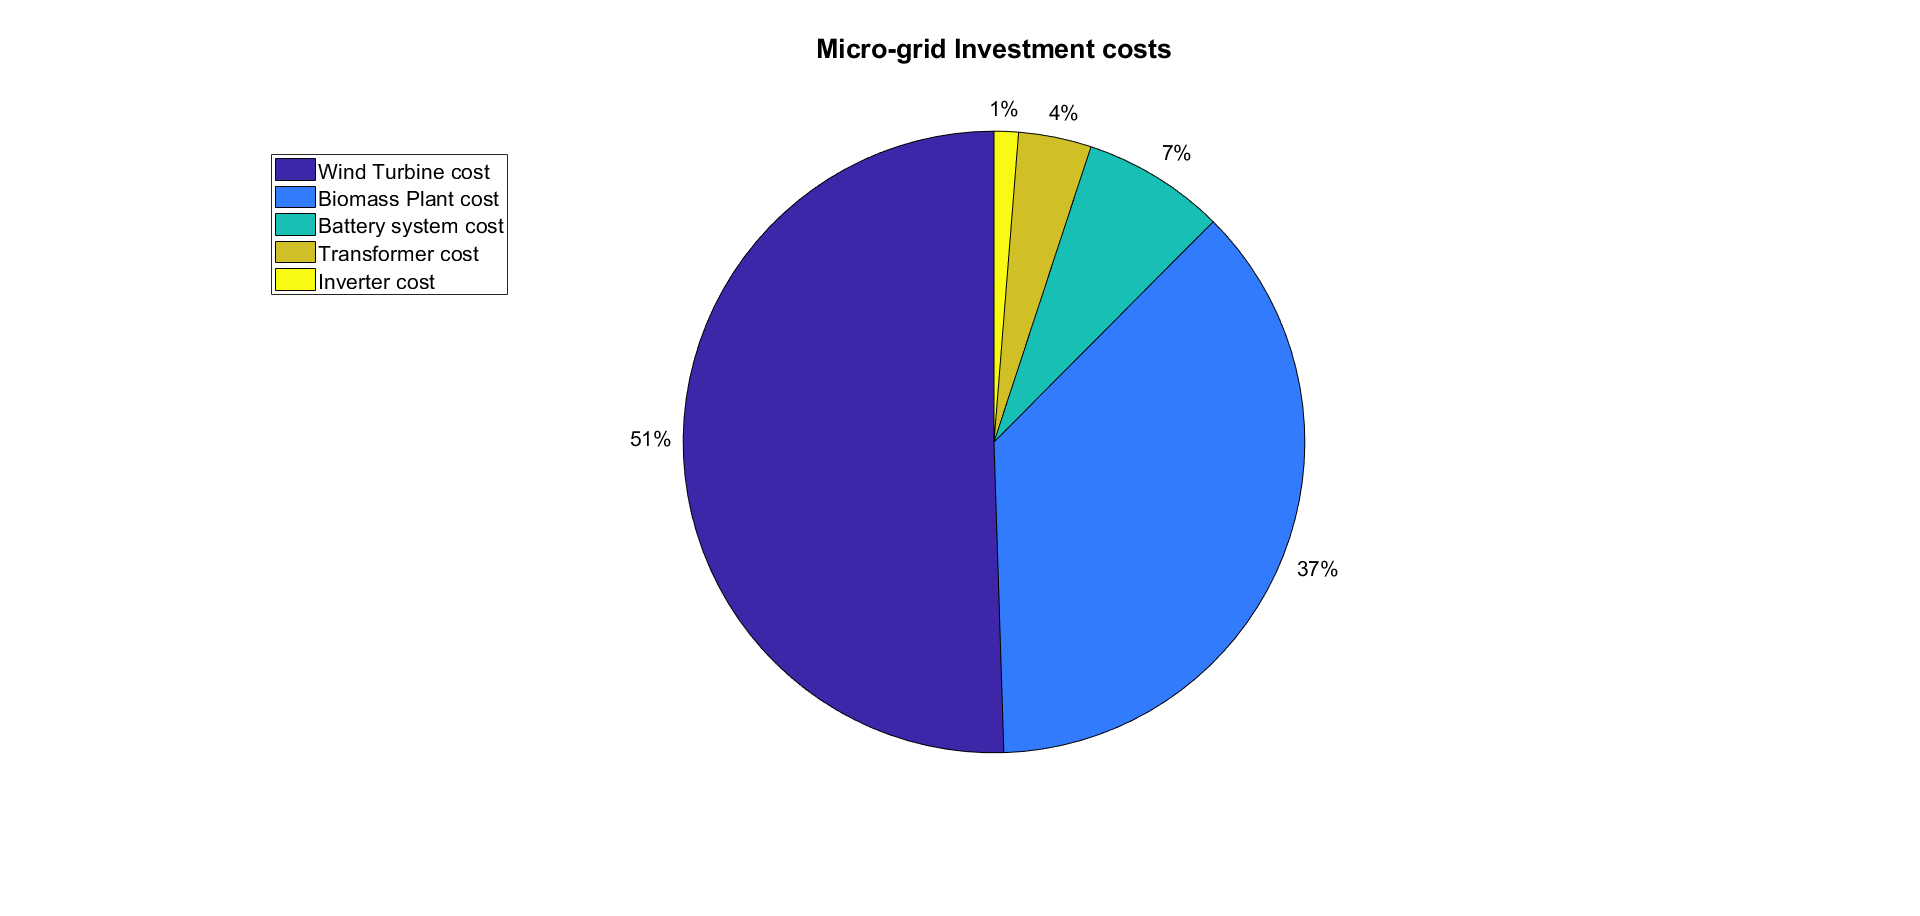
\includegraphics[width=1.1 \linewidth]{Final_report/Images/mginvest.png}
    \caption{Breakdown of investment costs for the micro-grid}
    \label{fig:mgtotal}
\end{figure}

\noindent The total investment cost for the micro-grid is $ Euro $ 118800. The Wind Turbine (primary) and Biomass Plant (secondary) generation units contribute to 90 \% of the total costs. The cost of the 50 KW wind turbine is of the order of $ Euro $ 60000.  For the biomass plant, the capital costs are estimated as a function of per KW installed capacity. This amounted to $ Euro $ 2000 per KW\citep{wbdg_2016}. The Battery system cost was $ Euro $ 8800\citep{doyle_2018}, and the additional costs taken into account for investments were for the 660 to 230 V step up transformer, and the bi-directional inverter for the battery system which were $ Euro $ 4500, and $ Euro $ 1500 respectively \citep{Alibaba}.

\subsection{LCOE calculation}
\label{LCOE}
The LCOE for the micro-grid was calculated using the following formula;
\begin{equation}
    LCOE = \frac{C_{invest}}{aE} + \frac{C_{O\&M}}{E} + \frac{C_{decom}(1+r)^{-T}}{aE}
\end{equation}
Where $ C_{invest}$, $ C_{O\&M} $, and $ C_{decom} $ correspond to investment, annual operation and maintenance, and decommissioning costs respectively. $ E $ pertains to the gross annual energy output of the generation units. In addition, the annuity factor $ a $is calculated using a discount rate $ r $. The life-time of generation units is given by $ T $.
For this project the following values were taken into consideration for LCOE calculation. The discount rate was taken as 3\% (considered as a recommended rate for energy projects according to \citep{IEA2015}), yielding an annuity factor of 18.9139. The annual energy yield $ E $ was computed for the Primary, Secondary generation sources. The Wind turbine annual energy output was calculated from the long term wind climate data and the power curve. For the biomass plant, the annual energy yeild was assumed to be equivalent to gross output per week repeated over the entire year. The battery discharge was appended to the total output of the grid, again assumed to be a constant repeated output for the entire year. The lifetime of generation units $ T $, was assumed to be 24 years. 

\noindent The costs considered for LCOE calculation are summarized in Figure \ref{fig:lcoe}. The individual breakdowns of the costs for the Wind turbine, and the biomass plant are given in Figure \ref{fig:w}, and \ref{fig:b}. For the wind turbine, operation and maintenance costs 

\begin{figure}[H]
    \centering
    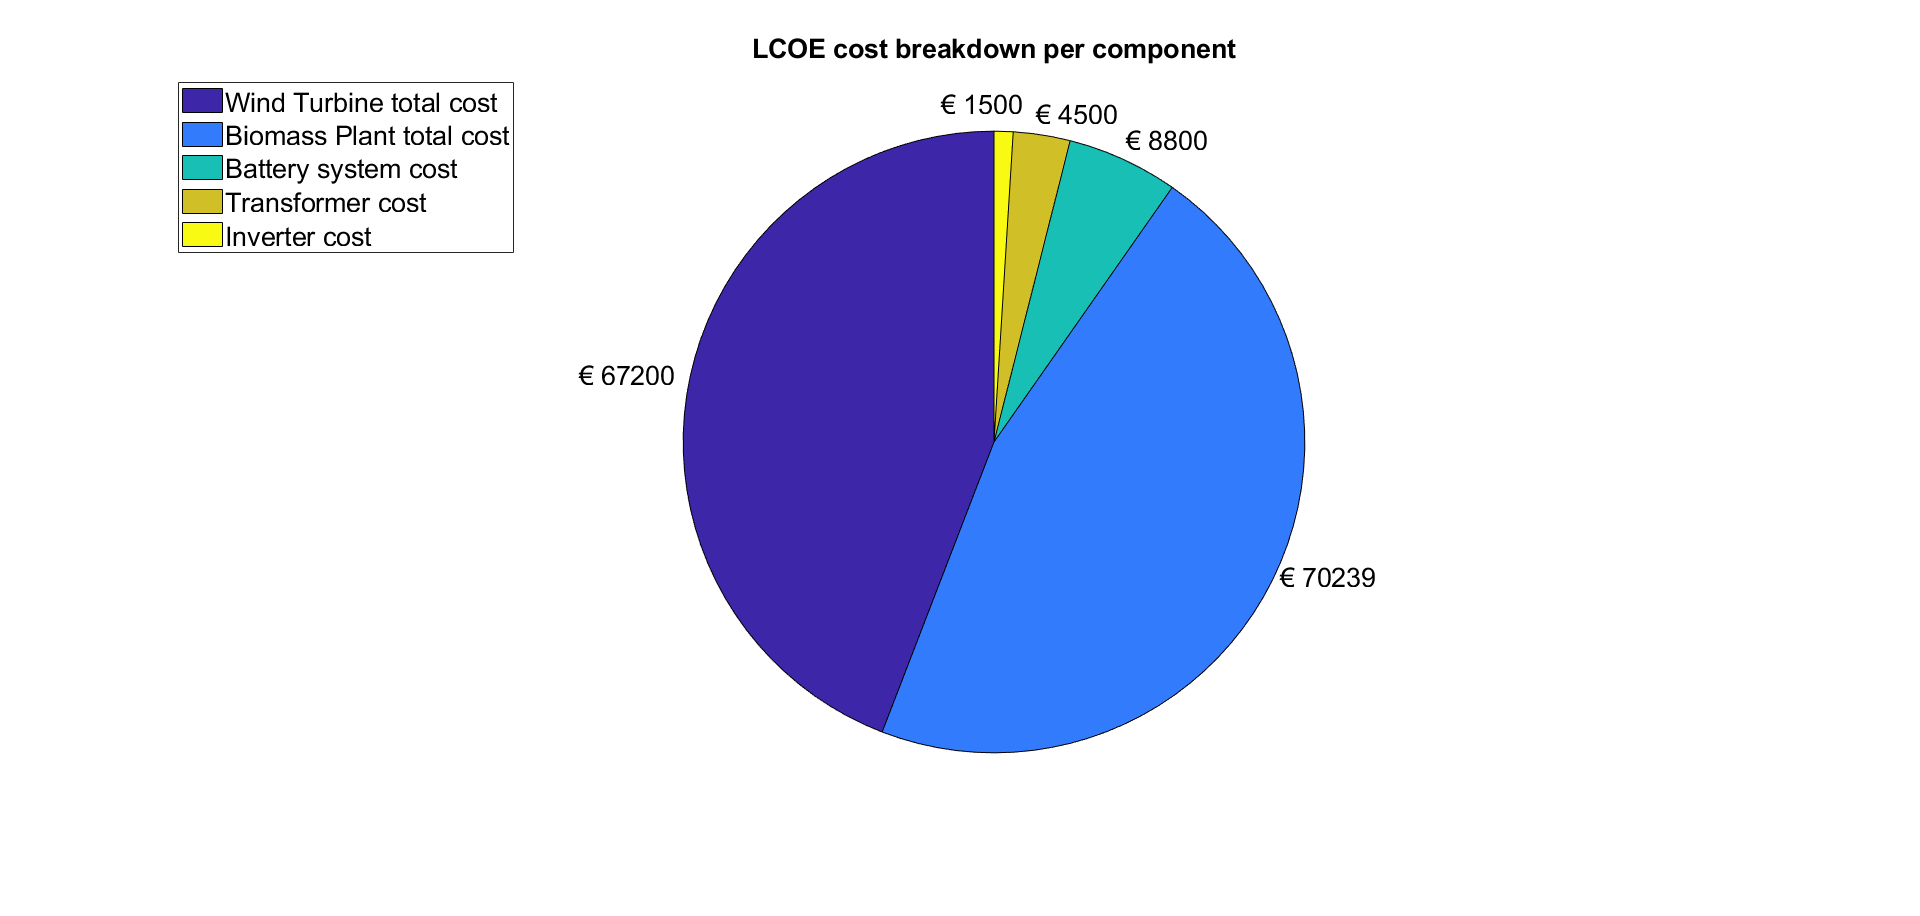
\includegraphics[width=1.1 \linewidth]{Final_report/Images/mgtotal.png}
    \caption{Breakdown of LCOE calculation costs per component}
    \label{fig:lcoe}
\end{figure}

\begin{figure}[H]
    \centering
    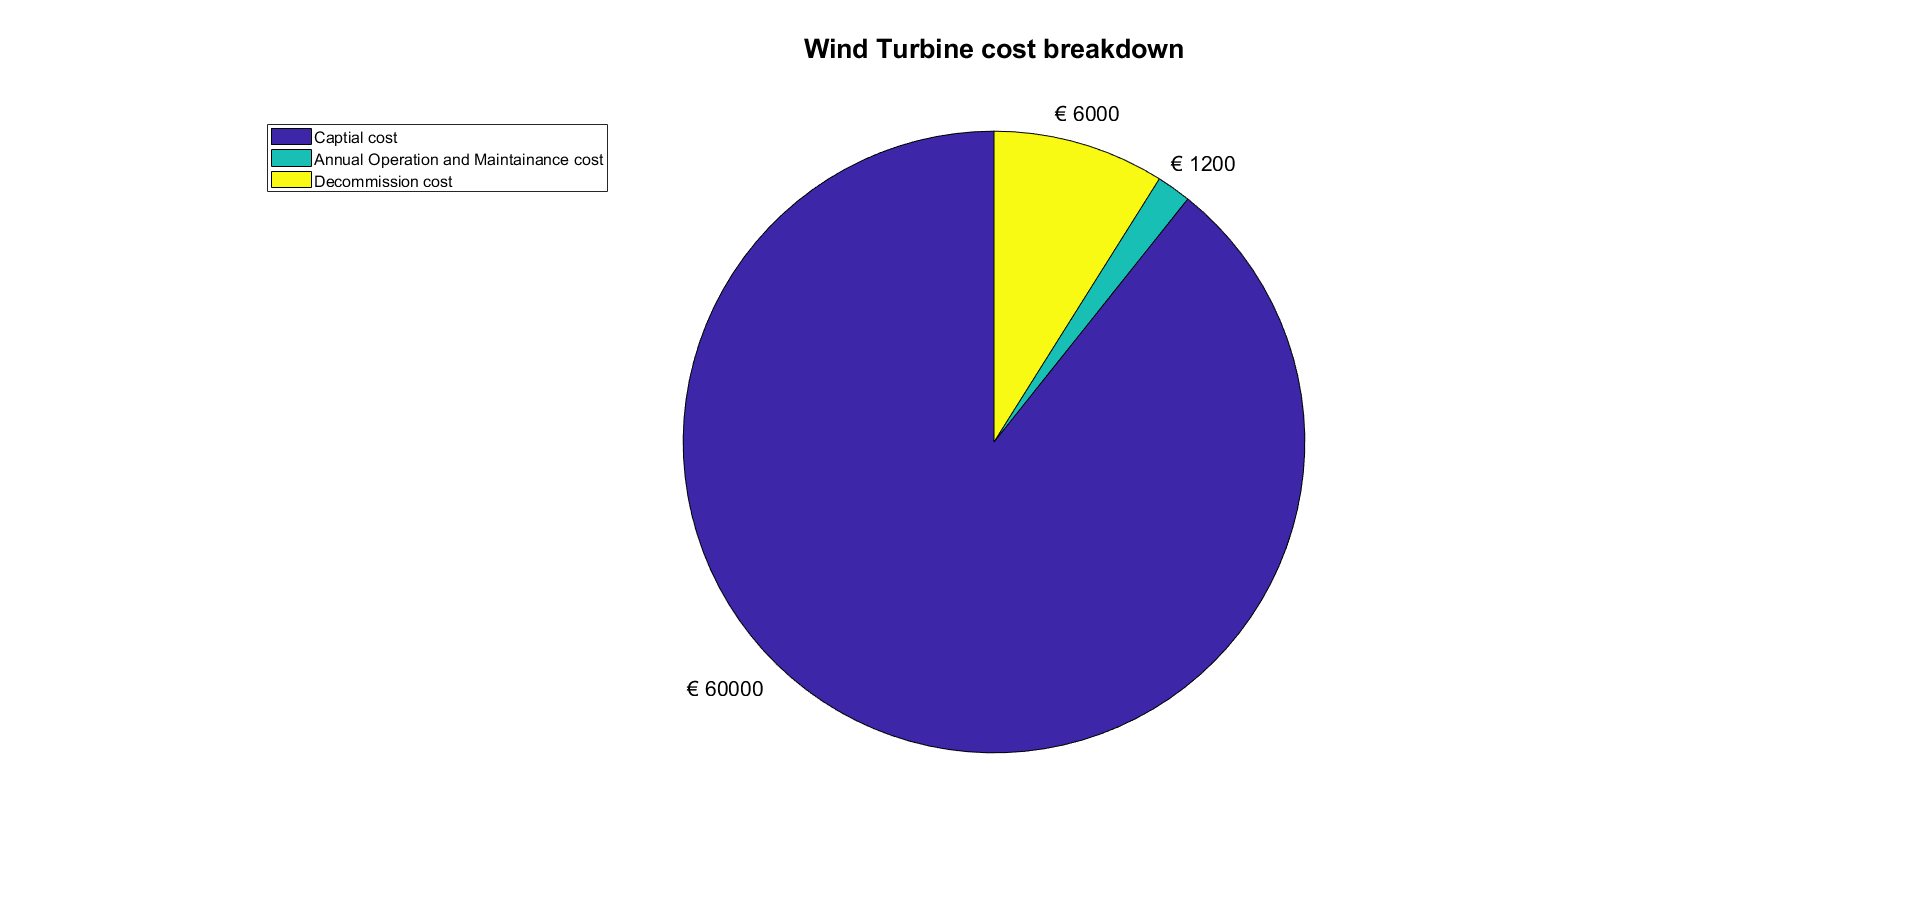
\includegraphics[width=1.1 \linewidth]{Final_report/Images/wtcost.png}
    \caption{Breakdown of Wind Turbine cost}
    \label{fig:w}
\end{figure}

\noindent The operation and maintenance, and decommissioning costs for the Wind Turbine are assumed to be 2\% and 10\% respectively, referenced from \citep{Weu2017}. This resulted in $ Euro $ 1200, and $ Euro $ 6000 respectively. 

\begin{figure}[H]
    \centering
    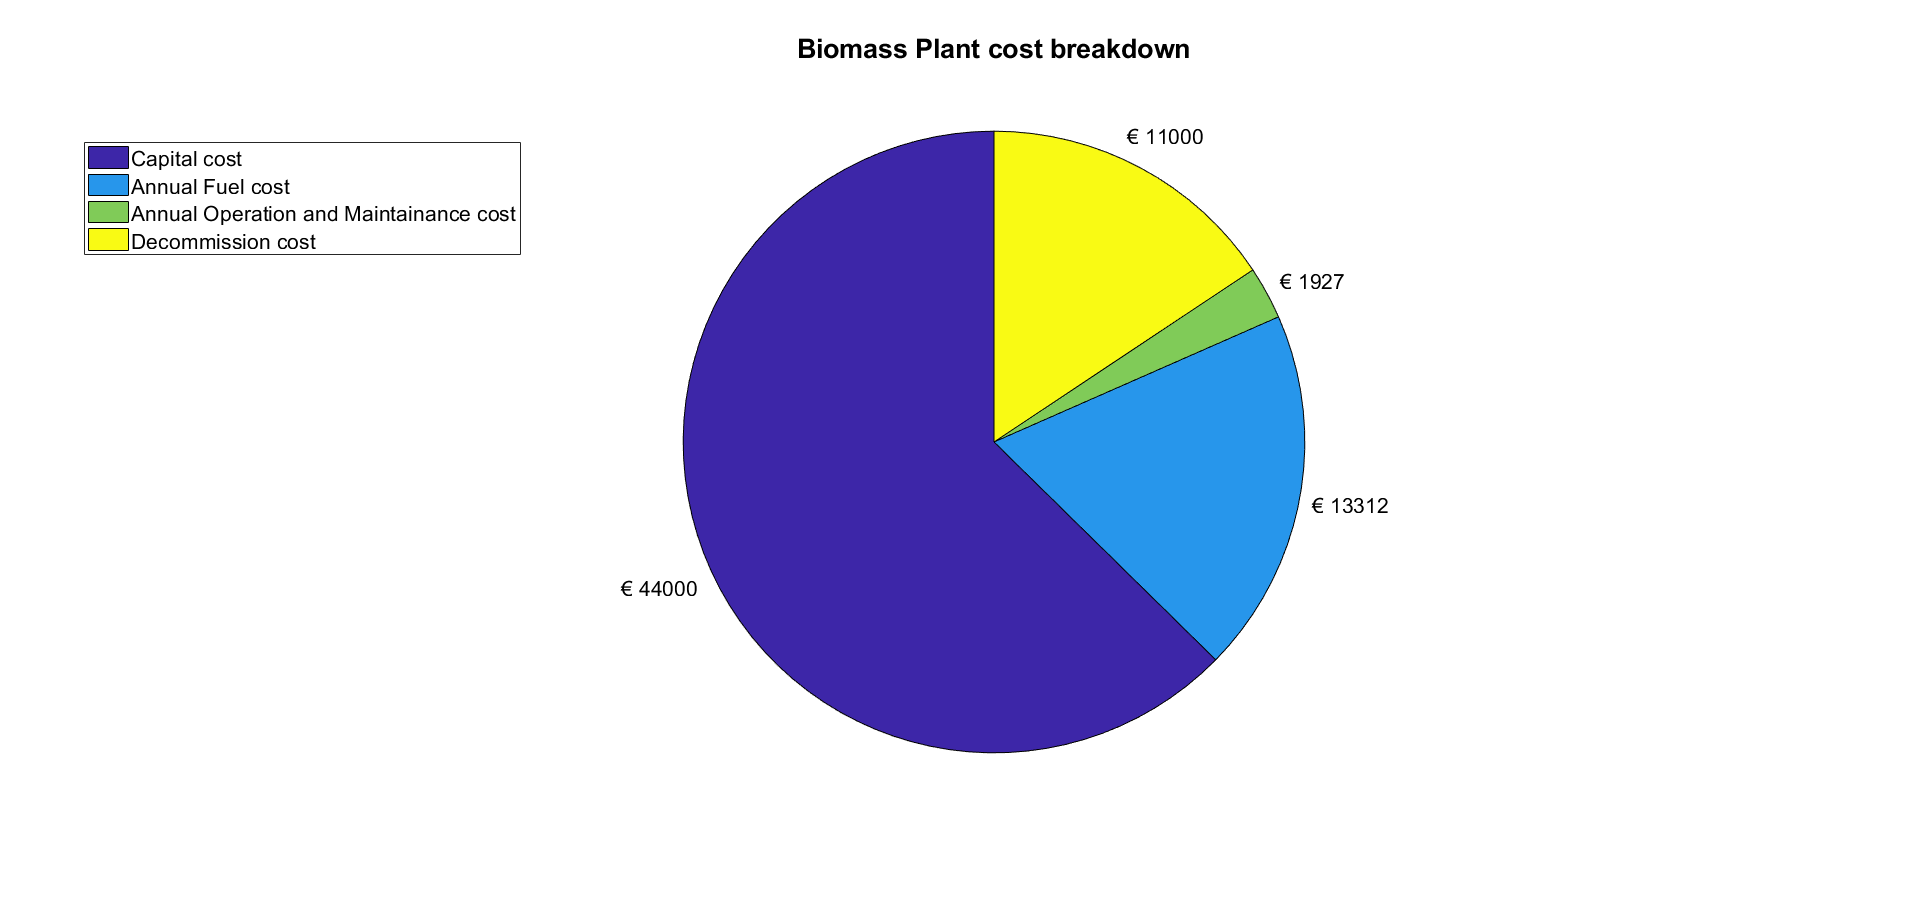
\includegraphics[width=1.1 \linewidth]{Final_report/Images/bmcost.png}
    \caption{Breakdown of Biomass Plant cost}
    \label{fig:b}
\end{figure}

\noindent The Biomass Plant additional costs have been broken down into annual operation costs, fuel costs, and decommissioning costs. The operation and maintenance costs were assumed to be 1\% of the rated energy produced per year. The fuel cost was estimated to be $ Euro $ 100 per ton \citep{beets_2017}, and the weekly fuel consumption was calculated to be 2.56 tons. Decommissioning costs were assumed to be 25\% of capital costs.

\noindent The total costs taken for the LCOE calculation as depicted in Figure \ref{fig:lcoe}, yielded a cost of 13.61 $ Euro $/KWh. It must be noted that a detailed break-up of the LCOE cost and procedure is given in the Appendix.

\subsection{Investment payback period}

Payback period in years for the micro-grid investment was calculated using the following relation: 
\begin{equation}
    Payback = \frac{C_{invest}}{LCOE*Load per year}
\end{equation}

\noindent The load per year was calculated assuming constant load profile for the entire year. The LCOE was used as the purchase cost for the electricity produced by the micro-grid. The payback period was thus found to be 5 years and 9 months.

%1.5 page
%G

\section{Environmental analysis}
This section deals with assessment of the environmental impacts of the micro-grid on two levels, namely the ecological costs associated with each component, and the ecological revenue of the project as a whole. In the first level, the impacts of each component in the project are discussed qualitatively. In the second level, the benefit of energy production from the micro-gird is assessed by referencing the relative CO2 emission from a natural gas plant of equivalent capacity. This is considered as the potential quantity of CO2 emission abated.

\subsection{Environmental impacts of the micro-grid components}

The potential effects on the environment by each component of the micro-grid are discussed here qualitatively.\\
\newline
Firstly, the effect of the Wind Turbine, is considered. The primary concern for allocating the location of wind turbine is proximity to households. This would require a noise constraint. On the otherhand, bird-strikes or the possibility for its occurrence need to be taken into account. The solution to these two obstacles lie in planning. 
\newline\\
Furthermore, for the biomass plant, the emissions produced during combustion of torrefied biomass has been considered. The main emission gases are $CH_{4}$,$N_{2}O$ and $CO_{2}$ which are lower than in case of natural gas\citep{derks_2018}.Further, the charcoal produced will be used as fertiliser for farmlands in Leeuwarden. Water supply for plant utilities such as cooling water and boiler water for the the steam generation, is taken from nearby streams in Leeuwarden connected to Wadden sea.   
\newline\\
Lastly, the battery system impacts can be summarized as the health and environmental effects of recovery of Vanadium pentaoxide $V_{2}O_{5}$ from vanadaium bearing slag due to its toxicity\citep{weber_peters_baumann_weil_2018}. However, these emissions are negligible as compared to previous mentioned sources.

\subsection{CO2 emission reduction}

The CO2 emission abatement with the micro-grid project can be measured by referencing the quantity of CO2 emitted from a natural gas plant of similar capacity. The annual energy yield of the micro-grid was calculated to be 126810 KWh. Assuming an emission rate of 0.502 kg/cubic metre, the quantity of CO2 abated was found to be 57.652 tons. This is after subtraction of the CO2 emission from the biomass plant which was calculated to be 6 tons\citep{derks_2018}.  


\noindent 
%1.5 page
%G

\section{Conclusion and recommendation}
%1 page 
%O
\subsection*{Conclusion}
The task of designing an islanded micro-grid involves the extensive survey of the location. Based on the location survey, wind turbine was found to be suitable as the primary source. Since the region is extensively agrarian, the logical choice for secondary source was a biomass plant. Due to the system isolation and instantaneous energy balance, Vanadium flow batteries were chosen. The initial sizing was based on the load profile provided (i.e average and peak loads). This sizing was revised after implementing the control philosophy. The reason being the sophisticated control, which tried to optimize the secondary generation. This significantly affected the sizing, and thus provided us with an insight into how the process of sizing is iterative. Simulation of the model was performed for a week under normal conditions. This was was followed by introduction of 3 scenarios, wherein the model performance and generation unit response was tested. The control strategy for the micro-grid was updated to accommodate preparedness for these scenarios. The simulation results showed that the mismatch, and the grid exchange was maintained as zero, even with the 3 scenarios. Finally, an economic and environmental assessment of the micro-grid was performed indicating the project feasibility and its impact on the environment. The economic assessment concluded that the project LCOE was reasonable for a micro-grid. The environmental assessment showed aspects to be considered for planning the components of the micro-grid, and the effective reduction in CO2 emissions were calculated in reference to a conventional generation plant. Overall, the planning, design, modelling, simulation, and economic assessment of the location specific micro-grid was performed, yielding a robust, and financially feasible project.

\subsection*{Recommendation}
The model tries to encompass most of the parameters of microgrids, but it could be enhanced by adapting the recommendations discussed below.

\noindent The component level modelling of each block could have more accurately predicted the microgrid performance.To optimise the secondary dispatch unit commitment can be implemented. An extensive power system dynamics analysis could support the control strategy. Inclusion of ancillary services would be beneficial is optimising the the sizing.The presence of reactive power control would also be benificial for the voltage stability. \\
Apart from technical recommendations it has been observed that the use of Biomass firing thermal plant as a secondary source is not the most economically viable option because of it's high operating costs.In addition to high cots the overall efficiency of the biomass plant is in the order of 5-6\% hence making it very inefficent and uneconomical to use. Thus, it is recommended to use more efficient technologies such as fuel cells and combined heat and power(CHP) to reduce the operating costs. Further, biomass energy can be converted to more feasible forms such as syngas and hydrogen which when combined with fuel cells can give much higher efficencies upto 60$\%$

\noindent For the economic assessment, accurate estimation of LCOE is subject to the assumptions made for discount rate, generation unit life, and breakup of costs. For this study, such assumptions were made yielding a semi-realistic result, and payback period. The Net Private Benefit was not calculated in this study for the individual project because a reliable estimate would require an accurate modelling of the cash flows over the life-time of the project, which was a limitation in this study. 


\newpage

\section*{Appendix}

\subsection*{Work chart}

\begin{table}[H]
\begin{tabular}{|l|c|c|c|c|c|c|c|}
\hline
\textbf{Names}     & \multicolumn{1}{l|}{\textbf{Primary}} & \multicolumn{1}{l|}{\textbf{Secondary}} & \multicolumn{1}{l|}{\textbf{Battery}} & \multicolumn{1}{l|}{\textbf{Control}} & \multicolumn{1}{l|}{\textbf{3 Phase}} & \multicolumn{1}{l|}{\textbf{Economics}} & \multicolumn{1}{l|}{\textbf{Environmental}} \\ \hline
\textbf{Rishikesh} & X                                     &                                         & X                                     & X                                     & X                                     &                                         &                                             \\ \hline
\textbf{Omkar}     & X                                     &                                         & X                                     & X                                     & X                                     &                                         &                                             \\ \hline
\textbf{Soham}     &                                       & X                                       & X                                     & X                                     &                                       &                                         & X                                           \\ \hline
\textbf{Gopan}     & X                                     &                                         & X                                     & X                                     &                                       & X                                       & X                                           \\ \hline
\end{tabular}
\end{table}